\documentclass[12pt]{extarticle}
\usepackage[utf8]{inputenc}
\usepackage{enumitem}
\usepackage{cite}
\usepackage{graphicx}
\usepackage{float}
\usepackage{listings}
\usepackage{hyperref}
\usepackage{siunitx}
\usepackage{microtype}
\graphicspath{{images/}}

\begin{document}

% --- COVER PAGE ---
\begin{titlepage}
    \centering
    % Title
    {\Large \textbf{Final Project I}\par}
    \vspace{1cm}
        
    {\Large \textbf{Planning AI Robot Arm Assistant for Tool Handling in Engineering Projects}\par}
    \vspace{1cm}
    
    % Faculty Logo
    
\includegraphics[width=0.25\textwidth]{cu_eng}\par\vspace{1cm}

    % Submitted to
    Submitted to the\\
    Project Committee appointed by the\\
    International School of Engineering (ISE)\\
    Faculty of Engineering, Chulalongkorn University
    \vspace{1cm}
    
    {\large \textbf{Project Advisor}} \\
    Asst.Prof.Paulo Fernando Rocha Garcia, Ph.D.
    \vspace{1cm}
    
    % Submitted by
    {\large \textbf{Submitted By}} \\
    \begin{tabular}{l l}
    Kanisorn Sangchai   & 6538020621 \\
    Methasit Boonpun    & 6538165021 \\
    Withawin Kraipetchara & 6538191221 \\
    Krittin Kitjaruwannakul & 6538007521 \\
    \end{tabular}
    \vspace{1cm}
    
    % Course, Faculty, University info
    1/2025: 2147416 Final Project I\\
Robotics and Artificial Intelligence Engineering (International Program)\\
International School of Engineering (ISE) Faculty of Engineering, Chualongkorn University

\end{titlepage}

\begin{abstract}
  Frequent tool switching in complex engineering projects disrupts workflows and reduces efficiency. Robotic assistants have been proposed as a solution for tool handling, yet many existing approaches rely heavily on end-to-end neural networks that lack interpretability and robustness in dynamic, unstructured environments. Recent research highlights the benefits of combining neural perception with symbolic reasoning, a paradigm known as neuro-symbolic artificial intelligence (NSAI). 
Togther with large language model (LLMs) and motion planning (TAMP) frameworks. These hybrid methods have shown function in enabling robots to understand natural language, reason about tasks, and execute reliable action in real-world scenario

The objective of this project is to develop a prototype of a Planning AI Robot Arm Assistant capable of supporting engineers task. The system aims to
\begin{enumerate}
  \item interpret natural language voice commands
  \item translate command into interpretable symbolic task plans
  \item detect, hold, and deliver engineering tool safely
  \item provide transparent reasoning process
\end{enumerate}
By focusing on interpretability, safety, and adaptability, the project addresses current limitations of existing robotic assistants and advances the development of collaborative human-robot systems.

The methodology involves integrating neural and symbolic AI within a system architecture. Speech recognition and natural language processing are used to understand user commands. These inputs are processed by a neuro-symbolic planning algorithm that generates task sequences. The system will be implemented and tested on a Universal Robots (UR) arm equipped with a gripper, depth camera, and microphone. Simulations and real-world experiment will validate the prototype to generalize to unseen scenarios and safely collaborate with human users in engineering environment  
\end{abstract}

\newpage
\tableofcontents

\newpage
\section{Background}

\begin{figure}[H]
    \centering
    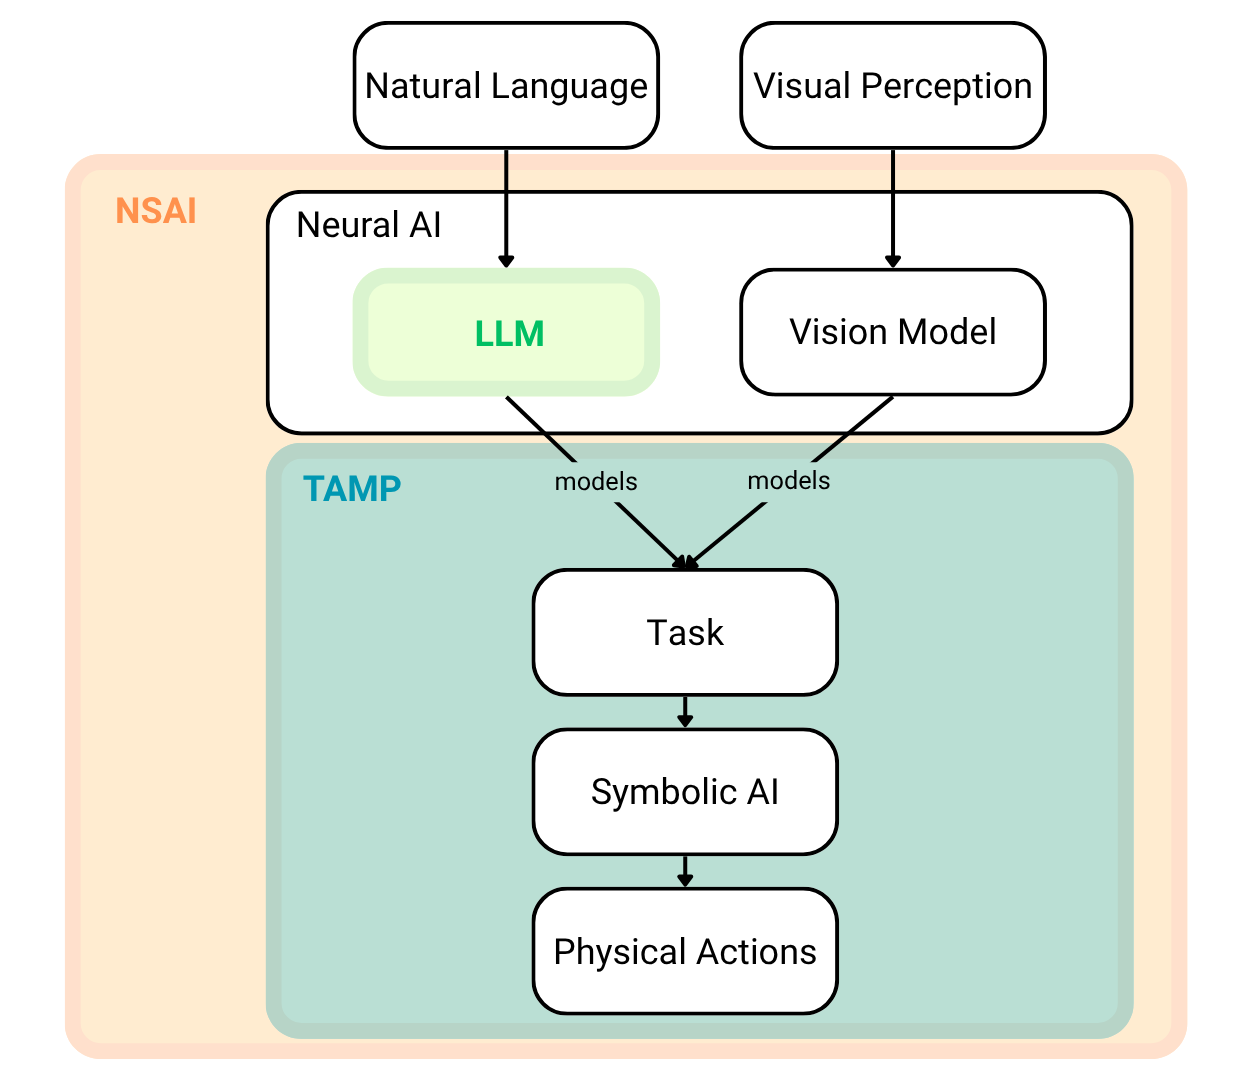
\includegraphics[width=0.7\linewidth]{images/background_graph.png}
    \caption{Relationship between TAMP, LLMs, and NSAI.}
    \label{fig:background-graph}
\end{figure}

Robotic assistants are increasingly seen as partners in human–robot collaboration settings, with the long-term goal of making them part of everyday work so that interacting with a robot feels as natural as working with another person. The present work takes a proof-of-concept perspective, focusing on how such systems might begin to support human tasks in controlled scenarios, while pointing toward the broader vision of seamless integration. Reaching this vision requires advances in robot manipulation and planning, supported by developments in task and motion planning (TAMP), large language models (LLMs), and neuro-symbolic artificial intelligence (NSAI). TAMP forms the classical foundation by linking high-level symbolic decisions with the physical feasibility of actions. Building on this, LLMs extend planning capabilities by using natural language to model tasks, decompose goals, and connect human instructions to symbolic representations. NSAI then combines these approaches, integrating the perceptual strengths of neural models with the structured reasoning of symbolic methods, offering a unifying paradigm that encompasses both TAMP’s grounding in feasibility and LLMs’ language-driven flexibility, as shown in Figure~\ref{fig:background-graph}.

\subsection{Robot Manipulation and Task Planning}
Historically, robot task execution was divided into two paradigms: AI task planning and robotics motion planning. Task planning generated abstract sequences of discrete actions using symbolic frameworks such as STRIPS or PDDL, while motion planning computed collision-free paths in continuous configuration spaces. This division proved sufficient in structured factory settings, where tasks and motions could be predefined, but inadequate in unstructured, human-centric environments~\cite{tamp},\cite{optimizatoin-and-motion-planning}. Early systems, such as Shakey the Robot, assumed high-level plans could always be refined into feasible motions, an assumption that rarely holds in practice~\cite{recent-trends-in-tamp}. The core difficulty was that symbolic plans often ignored geometric and kinematic constraints, producing strategies that were logically valid but physically infeasible. Task and Motion Planning (TAMP) overcame these limitations by formulating robot planning as a hybrid discrete–continuous search problem. By combining symbolic reasoning with geometric feasibility checks and introducing an intermediate level for selecting real-valued parameters such as grasps or placements, TAMP effectively bridged high-level planning with low-level execution, employing strategies such as backtracking refinement or interleaved search to prune infeasible plans~\cite{tamp}. Beyond feasibility, optimization-based formulations yield efficient trajectories, while learning-based methods accelerate feasibility checks, guide sampling, and adapt to novel settings~\cite{optimizatoin-and-motion-planning}. Crucially, TAMP allows robots to revise task strategies when geometric constraints block execution, enabling scalable planning in complex domains~\cite{recent-trends-in-tamp}.

\subsection{Large Language Models (LLMs) in Robot Manipulation}
Large Language Models (LLMs), particularly when augmented with visual reasoning as Vision-Language Models (VLMs), are increasingly central to robot manipulation, navigation, and broader embodied AI tasks, transforming complex initial states into desired goal states through sophisticated planning~\cite{plangenllm},\cite{eval-application-challenges-llms}. Beyond directly generating action sequences, LLMs also serve as Modelers, extracting and refining structured planning models such as Planning Domain Definition Language (PDDL) specifications from natural language, which mitigates challenges in long-horizon reasoning and enhances plan reliability~\cite{llm-as-planning-formalizers}. Leveraging world knowledge, reasoning, and decision-making, LLMs facilitate Task Modeling by converting human goals into initial and goal states and decomposing complex tasks into sequential, parallel, or recursive sub-goals. In robot manipulation, LLMs/VLMs improve handling of novel objects and generate motor or programmatic actions for perception, planning, and execution~\cite{plangenllm}. Furthermore,
their impact extends to human-robot interaction (HRI), enhancing intent interpretation and adaptability~\cite{eval-application-challenges-llms}.

Functionally, LLMs enable Domain Modeling, defining essential components like actions, preconditions, and effects, sometimes through demonstrations or iterative refinement~\cite{llm-as-planning-formalizers}, and integrate with sensory data to ground language understanding in spatial contexts, ensuring executable and robust plans. Integration with classical planners, hierarchical planning, and search algorithms allows LLMs to translate abstract goals into reliable action sequences guided by world models. Closed-loop feedback systems further enable dynamic adaptation, reducing hallucinations and improving task execution, while fine-tuning on planning-specific objectives enhances correctness and generalization~\cite{plangenllm},\cite{llm-as-planning-formalizers}. 

\subsection{Neuro-Symbolic Artificial Intelligence (NSAI) in Robot Manipulation}
Neuro-Symbolic Artificial Intelligence (NSAI) is an approach in robot manipulation that combines neural networks’ perceptual strengths with symbolic AI’s reasoning capabilities to create interpretable, interactive, and generalizable robotic agents in human-centric environments~\cite{enhancing-interpret},\cite{nsai}. NSAI enables robots to follow unconstrained natural language instructions for tasks like object picking, grasping, and multi-step manipulation such as pick-and-place or sorting~\cite{learning-neuro-symbolic}. Its architecture typically includes a hybrid scene encoder, neural language parser, reasoning/action primitives, symbolic program executor, and concept grounding modules. Language parsers translate instructions into executable symbolic programs, while scene encoders construct object-centric representations~\cite{enhancing-interpret},\cite{learning-neuro-symbolic}. Visual and spatial grounders match language concepts to objects, supporting generalization to unseen scenarios. Symbolic executors perform operations like filtering, querying, and executing manipulation actions~\cite{enhancing-interpret}, and simulators predict target locations for execution~\cite{learning-neuro-symbolic}. Training often uses weakly supervised, end-to-end curriculum learning with policy gradient methods~\cite{learning-neuro-symbolic},\cite{ns-vqa}. This modular design offers interpretability and enables interactive feedback. Challenges remain in integrating continuous neural models with discrete symbolic reasoning~\cite{nsai}, with future directions focusing on large language models for zero-shot parsing, vision-language models for grounding, and more complex logical structures for advanced planning~\cite{enhancing-interpret}.

\newpage
\section{Objectives}
Drawing from the prior examination of robotic manipulation through natural language command systems, there are multiple challenges and limitations, such as generalization, lack of interpretability, and handling complexity, that pose room for improvements. Thus, the project aims to tackle and explore these challenges and limitations by building a prototype of a personal AI assistant with a robotic arm that can:
\begin{enumerate}
  \item Understand natural language voice commands

  A primary challenge is enabling robots to effectively ground abstract semantic concepts in precise spatial reasoning from natural language. Current end-to-end neural networks, while capable of learning dexterous skills, often fail to generalize to new goals or quickly learn transferable concepts across tasks when confronted with language that introduces new concepts or slight variations (eg, distinguishing between "red pens" and "blue pens" without extensive new training data)~\cite{enhancing-interpret}. This highlights a core difficulty in how robots interpret the semantics underlying tasks from human instructions. Furthermore, past language-grounding methods for manipulation were often limited by object-centric representations and struggled to integrate perception and action cohesively based on linguistic input~\cite{cliport}. Overall, robots need to move beyond simple keyword recognition to a deeper, more generalizable understanding of human language in diverse, real-world contexts~\cite{enhancing-interpret},\cite{learning-neuro-symbolic}.

  \item Translate commands into symbolic task sequences

  Traditional Task and Motion Planning (TAMP) approaches specify tasks using formal representations like PDDL, but these require significant expertise and lack generalizability across different problems~\cite{code-as-symbolic-planner}. A promising solution involves neuro-symbolic AI, which combines the pattern recognition strengths of neural networks with the logical reasoning and structured knowledge of symbolic AI~\cite{nsai}. This hybrid approach allows for the explicit representation of the underlying reasoning process as symbolic programs, often using a Domain-Specific Language (DSL). Such disentanglement of perception (neural) from reasoning (symbolic) leads to systems that are more sample-efficient , can generalize to unseen concept-task combinations, and enable deeper, compositional, and hierarchical reasoning over abstract concepts derived from instructions~\cite{enhancing-interpret}. Recent advancements has highlighted an alternative approach by exploring guiding LLMs to directly generate code that serves as the robot's TAMP planner and checker , integrating symbolic computation into the planning process while maintaining broad generalizability~\cite{code-as-symbolic-planner}.

  \item Detect, grasp, and deliver engineering tools safely to the user

  Accomplishing this requires overcoming challenges in precise spatial reasoning and robust interaction with objects in dynamic, unstructured environments. Current systems, even those showing promise in semantic understanding, may still struggle with fine-grained manipulation that demands high spatial precision, such as handling deformable objects or specific placements. Generalization to novel object instances that were not part of training data remains a hurdle, with models sometimes exploiting biases rather than truly grounding instructions~\cite{cliport}. The process involves object detection, instance segmentation, and grasp synthesis to identify and physically interact with items~\cite{enhancing-interpret}. Furthermore, ensuring safety during physical interaction is paramount, requiring rigorous validation and addressing issues like collision avoidance and potential biases from pre-trained models that could lead to harmful actions. The "sim-to-real" gap also means that models trained in simulation may require substantial fine-tuning for robust real-world performance~\cite{enhancing-interpret},\cite{cliport}.

  \item Provide interpretable task plans that users can inspect, adjust, or correct

  This addresses the critical problem of "black box" AI, where purely neural systems lack transparency and the ability to explain their decisions. This opacity makes it challenging for non-expert users to diagnose and correct errors in a robot's behavior. Neuro-symbolic AI explicitly tackles this by disentangling reasoning from visual perception and language understanding, leading to fully transparent and interpretable reasoning processes. By generating explicit symbolic programs that represent the robot's plan as a sequence of logical steps, the system provides a formal, interpretable representation of its decision-making. This interpretability is crucial for human-in-the-loop interaction , allowing users to understand why a robot performs certain actions, inspect the generated task plans, and provide targeted feedback or corrections when a failure occurs. The ability to communicate about failures and ambiguities in a dialogue setting significantly enhances usability and trust in autonomous systems~\cite{enhancing-interpret},\cite{nsai}.



\subsection*{Evaluation Metrics and Benchmarks}

To demonstrate successful end-to-end handover, the system must integrate language understanding, symbolic planning, perception, and grasping into a reliable pipeline. Recent studies show that robot-to-human tool handover can reach around 92.5\% success in simulation for construction tools~\cite{iaarc2025_handover}, while sim-to-real grasping frameworks report 90--97\% success depending on object familiarity~\cite{mogpe2022},\cite{grasping2023}. Performance is typically lower for novel or cluttered settings, highlighting the importance of generalization.  

Timing benchmarks suggest that simple object handovers can be completed in 8--10 seconds~\cite{handover2024_fast}, though more complex engineering tools may reasonably require up to 15 seconds. Based on these findings, this project defines its main performance goal as achieving \textbf{$\geq90\%$ success over 60–80 trials}, with \textbf{completion within 15 seconds} and \textbf{minimal disturbance} $\leq\SI{2}{\centi\meter}$ to non-target tools.


\end{enumerate}

\newpage
\section{Literature Survey and Review}

\subsection{Existing Solutions for Robot Manipulation through Natural Language Instructions}

\subsubsection{Voice Control and Multimodal Speech Recognition for Robot Manipulation}

Voice-based interaction provides a natural interface for instructing robots, and Automatic Speech Recognition (ASR) forms the foundation of such systems. Early approaches relied on keyword spotting and grammar-based recognition, which worked reliably for simple commands in controlled environments~\cite{smith2015voice}. However, these systems often fail under noisy conditions or when commands are ambiguous, motivating the shift toward data-driven neural methods.

Recent studies have addressed ASR robustness by incorporating sequence-to-sequence parsing with noise injection, allowing semantic parsers to tolerate ASR errors commonly encountered in service robotics~\cite{tada2020robust}. Similarly, distributed architectures have been proposed, such as using an Android device for speech recognition coupled with a lightweight microcontroller (ESP32) for actuation, achieving low-latency, real-time control even in noisy environments~\cite{gupta2025speech}.

Beyond speech-only systems, multimodal ASR approaches integrate visual, gestural, or haptic information to improve recognition and grounding. For instance, the Vision-Language-Action (VLAS) framework combines speech and visual inputs to interpret commands in dynamic environments, enabling context-aware robot manipulation~\cite{yu2020vlas}. Other multimodal methods leverage gaze tracking or environmental cues to disambiguate spoken instructions, reducing errors and improving task performance~\cite{liu2021multimodal}.

Despite these advances, limitations persist. ASR systems still degrade in real-world noisy conditions, while multimodal approaches often require expensive sensors or large-scale datasets, limiting general deployment~\cite{liu2021multimodal}. Moreover, most works focus on recognition accuracy, with fewer studies addressing usability, user experience, or trust in human-robot interaction. These gaps highlight the need for solutions that are both technically robust and practically deployable in everyday environments.



\subsubsection{Robot Planning}

Recent advances in robot planning and manipulation have increasingly focused on leveraging large vision-language-action (VLA) models to enable robots to interpret high-level instructions and execute complex tasks. Rather than treating perception, reasoning, and control as isolated problems, the field has shifted towards integrated approaches where natural language commands can directly guide manipulation policies. These models combine multimodal perception, grounded reasoning, and action generation, allowing robots to handle tasks ranging from simple pick-and-place to multi-step assembly.

Two principal architectural paradigms have emerged: monolithic models and hierarchical models~\cite{vla-in-robot}. Monolithic models aim to jointly optimize perception, reasoning, and control in a single pipeline. Within this category, single-system designs treat robot actions as autoregressively generated tokens, enabling strong semantic generalization from large-scale pretraining but suffering from slow inference and limited interpretability. Dual-system designs mitigate these issues by pairing a slower, deliberative planner with a fast execution module, though they introduce challenges in synchronization and integration.

Hierarchical models, by contrast, explicitly decouple high-level planning from low-level execution. They produce interpretable intermediate representations—such as subtasks, spatial keypoints, or structured programs—that bridge natural language instructions and executable control policies. This modularity improves transparency and supports long-horizon reasoning, enabling decomposition of complex tasks into manageable steps. Approaches like program-based planning connect natural language to symbolic structures or robot APIs, balancing interpretability with execution fidelity.

Across both paradigms, several strategies address the challenges of efficiency, generalization, and robustness~\cite{vla-in-robot}. To reduce inference latency, work has explored parallel decoding, compressed action tokenization, and lightweight architectures. To improve adaptability, VLA models increasingly incorporate predictive world models, richer perception modalities (e.g., depth, tactile, and temporal cues), reinforcement learning for dense feedback, and human video data for cross-domain knowledge transfer. Safety mechanisms such as adaptive planning and dynamic risk assessment further strengthen reliability in unstructured environments.

Within this broader landscape, hybrid neuro-symbolic approaches demonstrate how symbolic reasoning can be combined with learned perception and language grounding. By integrating interpretable intermediate structures with robust neural representations, these systems can generalize to novel tasks while maintaining transparency and interactive error correction~\cite{enhancing-interpret},\cite{learning-neuro-symbolic}. Program-synthesis-based methods extend this paradigm, treating generated code as an evolving hypothesis that can be validated, repaired, and refined through execution feedback~\cite{hycodepolicy},\cite{code-as-policies},\cite{code-as-symbolic-planner}. Other efforts leverage large language models to interface directly with planning and control APIs, reducing reliance on end-to-end policy generation while increasing flexibility and autonomy~\cite{audere}.

Taken together, these developments highlight a trend toward unifying natural language, perception, and action in robotic planning. The field is moving from narrow, task-specific systems toward general-purpose agents capable of robust, interpretable, and scalable manipulation across diverse real-world settings.


\subsection{Existing Technology for Robot Manipulation through Natural Language Instructions}

\subsubsection{Voice Control and Multimodal Speech Recognition for Robot Manipulation}

Voice Control Systems (VCS) have transformed human-computer interaction by enabling intuitive, hands-free communication through natural language commands. Traditionally, VCS relies on Automatic Speech Recognition (ASR) to transcribe speech into text and Natural Language Processing (NLP) to interpret and execute instructions. These systems are widely used in digital assistants, smart homes, and IoT devices, enhancing accessibility, convenience, and efficiency in everyday tasks. In robotics, VCS lowers barriers to interaction by allowing users, including children and individuals with limited mobility, to control robots naturally through speech~\cite{vcs}. Despite these advantages, traditional ASR systems remain limited in noisy, ambiguous, or dynamic environments. They often struggle with fine-grained contextual information or visually grounded references, which are critical for successful robot manipulation. To address these challenges, multimodal ASR has emerged as an extension of VCS, incorporating both speech signals and visual context to ground linguistic input in the robot’s perceptual environment~\cite{Chang2023},\cite{multi}.

\textbf{Core Architecture of Multimodal ASR:}
\begin{itemize}
    \item \textbf{Speech Encoder:} Extracts audio features from spoken instructions, often using pre-trained models such as wav2vec 2.0.
    \item \textbf{Visual Encoder:} Processes visual observations from the robot’s environment (e.g., CLIP-ViT).
    \item \textbf{Language Decoder:} A Transformer-based decoder that jointly attends to both speech and visual features to generate accurate transcriptions.
\end{itemize}

By combining speech with visual context, multimodal ASR achieves higher transcription accuracy, especially for visually salient words such as object names or spatial instructions. It also improves task success rates by reducing errors from misheard commands and generalizes better across new environments and diverse speakers. Benchmarks such as ALFRED have demonstrated that multimodal ASR enables robots to more reliably follow natural language instructions in simulated household environments~\cite{vcs},\cite{Chang2023},\cite{multi}. By uniting the accessibility of traditional VCS with the robustness of multimodal ASR, robots gain the ability to interpret and execute commands more effectively in uncertain and dynamic conditions. This evolution marks a critical step toward human-robot interaction that is both natural and contextually grounded~\cite{vcs},\cite{Chang2023},\cite{multi}.

\subsubsection{Robot Planning}

Robot manipulation tasks, particularly in unstructured human environments, necessitate that robots can understand and execute natural language instructions from non-expert users~\cite{cliport}. Historically, robot planning relied on segregated high-level artificial intelligence (AI) task planning and low-level motion planning, with traditional methods often using hand-coded symbols or relying on strict hierarchical decompositions~\cite{learning-neuro-symbolic},\cite{code-as-symbolic-planner}. However, these approaches struggled to effectively combine discrete task decisions with continuous geometric and kinematic considerations, limiting their applicability in dynamic, human-centric settings~\cite{cliport},\cite{code-as-symbolic-planner}.
Recent advancements have led to diverse implementations and approaches, broadly categorized as:

\begin{enumerate}[label=\Roman*.]
    \item \textbf{Traditional / Early Language Grounding} \\
Traditional methods typically map natural language phrases to pre-defined symbolic representations of robot states and actions, assuming a symbolic description of the environment and actions. They often rely on symbols hand-coded by domain experts~\cite{optimizatoin-and-motion-planning} or logical parses that translate language into motion constraints or control actions, and generally lack the flexibility to autonomously learn task semantics~\cite{learning-neuro-symbolic}. While these methods provide clear symbolic interpretability, they are inherently limited in their generalizability—new goals (e.g., switching from red pens to blue pens) require new training or explicit user input~\cite{ns-vqa}.

Interpretability is high since the reasoning is explicit and symbolic, but they often fail to integrate discrete task planning with continuous motion feasibility~\cite{tamp}, restricting use in dynamic, real-world settings. Data efficiency is poor, as pre-annotated datasets are needed to map phrases to symbols. Additionally, scalability is limited since symbolic operators are predefined, and the frameworks cannot easily adapt to unseen tasks.

    \item \textbf{Language-Conditioned End-to-End Systems (e.g., CLIPORT)} \\
These systems combine large-scale pre-trained vision-language models (like CLIP, for broad semantic grounding—the “what”) with architectures specialized for spatial precision (like Transporter—the “where”). Transporter Networks are highly sample-efficient, end-to-end models for robotic manipulation that avoid object-centric assumptions, exploiting spatial symmetries and generalizing well to unseen objects and configurations~\cite{transporter}. CLIPORT builds on this by integrating language-conditioned policies and semantic understanding via a two-stream design, enabling grounding of categories, shapes, colors, and text attributes without requiring hand-designed perception pipelines. They show strong data efficiency, can learn multi-task policies, and generalize across seen and unseen semantic concepts, transferring learned attributes to new tasks~\cite{cliport}.

However, challenges remain. CLIPORT struggles with fine-grained reasoning about relationships (e.g., “middle square hole” with unseen shapes), counting, or verb-noun generalization beyond training data. Its execution is limited to open-loop pick-and-place primitives, making it brittle in dynamic or dexterous tasks. Interpretability is partial: while the semantic prior is clear, the underlying reasoning process remains mostly opaque. Calibration errors or biases in training data can degrade performance, and extending to high-DOF manipulation is non-trivial~\cite{cliport}.

    \item \textbf{Neuro-Symbolic Approaches} \\
Neuro-symbolic methods integrate neural perception modules with symbolic reasoning engines. They often translate natural language into executable symbolic programs composed of both neural (e.g., visual grounding) and symbolic (e.g., counting, logic) primitives. This enables them to combine robust perception with transparent, structured reasoning. Examples include the DeepSym framework for autonomously discovering symbols, neurosymbolic architectures for coupling vision and reasoning, and program-generating models for manipulation~\cite{nsai}.

NSAI systems enhance interpretability, robustness, and trustworthiness, while also facilitating learning from less data. By disentangling perception and language understanding (neural) from reasoning (symbolic), neurosymbolic systems offer a formal, interpretable representation of the underlying reasoning process~\cite{enhancing-interpret}. They are also highly sample-efficient, capable of learning from weak or “natural” supervision (initial/final states rather than dense annotations)~\cite{nsai},\cite{learning-neuro-symbolic}.

However, limitations include reliance on fixed domain-specific languages (limiting concept coverage), susceptibility to perception errors in cluttered scenes, and difficulty scaling to more complex logic (loops, conditionals)~\cite{enhancing-interpret},\cite{learning-neuro-symbolic}. Integration of neural and symbolic modules introduces computational challenges such as state-space explosion and longer training times, and standardization across frameworks remains an open problem~\cite{nsai}.

    \item \textbf{Large Language Model (LLM)-Based Approaches} \\
LLM-based methods leverage the broad commonsense reasoning of large pre-trained language models for robot planning. Some approaches map natural language into symbolic planning representations (e.g., Text2Motion~\cite{text-2-motion}), while others use LLMs to choose from pre-defined primitives (e.g., Code-as-Policies~\cite{code-as-policies}). A recent paradigm, Code-as-Symbolic-Planner, queries the LLM to generate executable code that acts as both the planner and verifier, explicitly integrating symbolic computation~\cite{code-as-symbolic-planner}.

Their generalization is strong due to pretraining on vast text/code datasets. LLMs provide natural language transparency and can even generate interpretable code that reflects explicit reasoning chains~\cite{code-as-symbolic-planner},\cite{code-as-policies}. Data efficiency benefits from pretraining, though TAMP-specific fine-tuning or self-checking guidance frameworks are often required~\cite{plangenllm}.

However, challenges include brittleness in complex optimization scenarios, inconsistency in generated code, and performance degradation with increasing task complexity. Earlier LLM methods that lacked symbolic computation were unreliable for tasks with numeric constraints~\cite{code-as-symbolic-planner}. Even with code generation, outputs may be suboptimal or erroneous, requiring iterative refinement. Furthermore, real-world translation of problems into solvable code remains difficult, and generated code can introduce execution risks~\cite{plangenllm}.

\item \textbf{Vision-Language-Action (VLA) Models} \\
VLA models couple perception, language understanding, and control to enable robots to follow high-level human instructions. They leverage large vision-language models for open-world generalization, hierarchical planning, and knowledge-augmented reasoning.

Two main paradigms exist. Monolithic models integrate perception, reasoning, and control in a single pipeline, offering strong generalization but facing slow inference and limited interpretability. Hierarchical models decouple planning from execution by producing explicit intermediate outputs (e.g., subtasks, keypoints, or code), which improves modularity, transparency, and long-horizon reasoning but increases system complexity.

Efficiency and robustness are enhanced through parallel decoding, lightweight architectures, action token compression, world-model integration, advanced multimodal perception, reinforcement learning, and safety-aware planning. Remaining challenges include inference bottlenecks, synchronization between modules, and robustness across embodiments~\cite{vla-in-robot},\cite{vla}.

\end{enumerate}

\subsection{Conclusion}
The field of robot manipulation and planning through natural language is moving towards the main goal of enabling robots to seamlessly translate human intent into precise, executable actions. Current progress demonstrates the promise of LLMs and MLLMs in bridging abstract linguistic instructions with the concrete demands of real-world robotics. By combining high-level semantic understanding with fine-grained spatial reasoning, generating interpretable code as flexible policies, and leveraging neuro-symbolic reasoning for systematic generalization, researchers are building the foundations for robots that can adapt to diverse tasks and environments. These approaches, when coupled with modular design and iterative feedback loops, highlight a path toward truly intelligent and collaborative robotic assistants.

For this project, we aim to contribute to this progress by addressing some of the key limitations in the field. In particular, we will explore extending manipulation capabilities toward more complex object handling based on high-level commands, while also investigating methods for improving robustness and adaptability under real-world uncertainty. We see opportunities in integrating neural and symbolic reasoning, advancing perception systems for richer grounding, and experimenting with human-in-the-loop strategies for preference alignment and safe deployment. By targeting these areas, We hope to push the field closer to building robots that are not only capable and efficient but also trustworthy collaborators in human-centered environments.

\newpage
\section{Project Concept Development with Core Technology}

\begin{figure}[H]
    \centering
    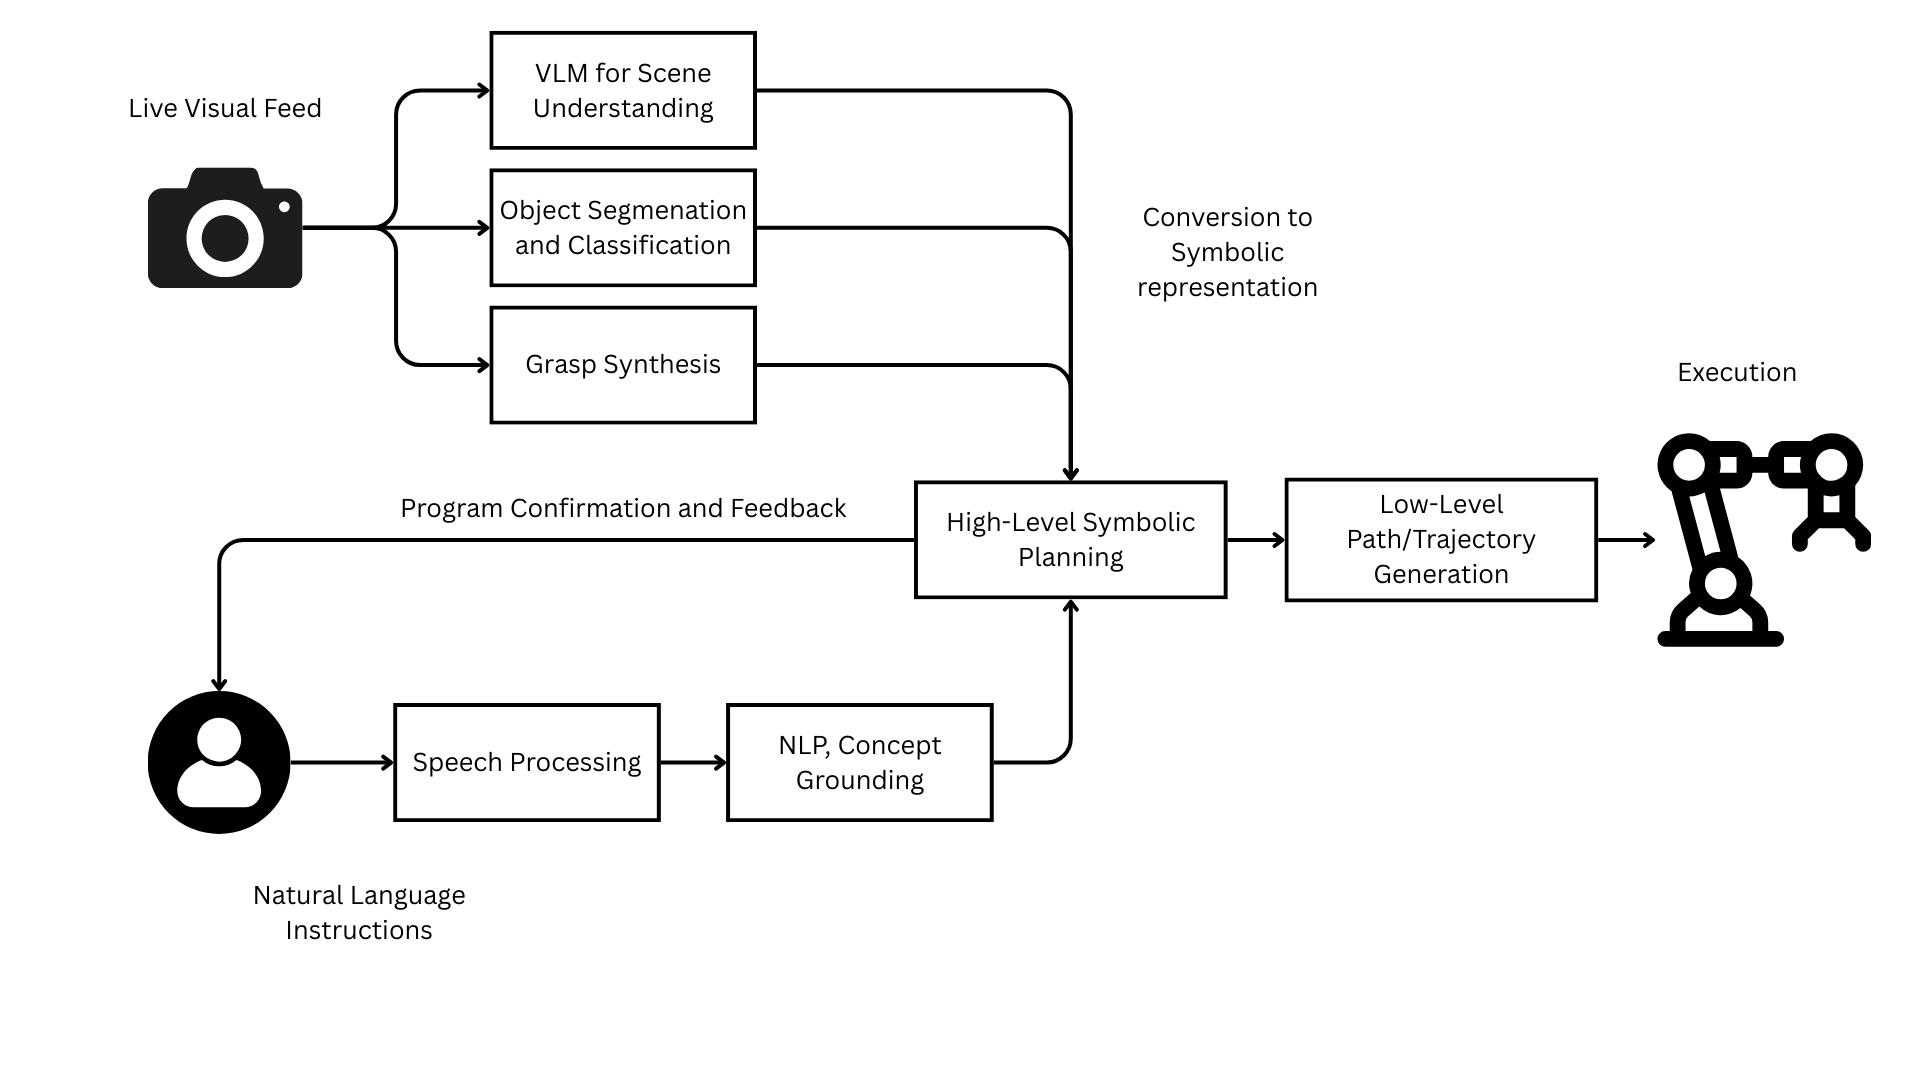
\includegraphics[width=\linewidth]{images/System_Architecture_Overview.png}
    \caption{System Architecture Overview}
    \label{fig: architecture overview}
\end{figure}

The project combines:
\begin{itemize}
    \item \textbf{Neural AI}: Object detection, segmentation, grasp synthesis, automatic speech recognition, and natural language understanding.
    \item \textbf{Symbolic AI}: Constraints enforcement to ensure executability. Path and trajectory generation.
    \item \textbf{Robotics}: A robot arm with a gripper executing precise manipulation under safe handover protocols. 
\end{itemize}
This neuro-symbolic hybrid design ensures adaptability, efficiency, and user transparency. \\

\textbf{\underline{Overall Workflow:}}
\begin{enumerate}
    \item Users instruct the robot through high level, natural language, vocal commands.
    \item The vocal command is converted into text using Automatic Speech Recognition (ASR) pipeline.
    \item Semantics and discrete concepts are extracted from the text commands using Natural Language Processing (NLP) techniques, resulting a detailed description (for LLMs).
    \item The current state of the work area is perceived through a camera.
    \item The live visual feed is processed by applying object detection, segmentation, grasp synthesis, and visual understanding.
    \item Visual and textual information are converted into symbolic representation by utilizing LLMs with access to visual perception tools and query users for additional details.
    \item The symbolic high-level planner decomposes the high-level task into sequential sub-tasks.
    \item The user can confirm, reject, or adjust the program proposed by the algorithm. Creating a closed-loop feedback system that allows more control.
    \item Once a plan is confirmed by the user, each sub-task is executed.

\end{enumerate}

\subsection{The Current Development of the Project}

\subsubsection{Speech}
To establish a robust Automatic Speech Recognition (ASR) foundation for robot manipulation, a \textbf{real-time speech-to-text system} was developed and implemented as a \textbf{ROS2 node} using the \textbf{AssemblyAI API}. Unlike the initial prototype, which processed pre-recorded audio inputs such as \textit{harvard.wav}, the new system continuously captures live audio streams, transcribes them in real time, and publishes the recognized text for downstream processing. Additionally, if no speech input is detected for \textbf{three seconds}, the node automatically stops listening and outputs the most recent transcription result.

AssemblyAI serves as the core transcription engine, leveraging advanced \textbf{deep learning models} to convert speech into accurate text through a structured pipeline that includes \textit{feature extraction}, \textit{acoustic modeling}, \textit{language modeling}, and \textit{decoding}. These stages enable the system to handle diverse speech patterns and environmental noise effectively. Furthermore, post-processing mechanisms such as punctuation restoration, capitalization, and disfluency removal enhance the clarity and readability of the generated text.

As illustrated in Figure~\ref{fig: ASR_Pipeline.png}, the implemented ASR node operates through a continuous loop of capturing live microphone input, sending it as a transcription job, polling for recognition results, and checking for further user input. When no speech is detected within three seconds, the node terminates the current session and publishes the final transcription output. This workflow provides a \textbf{modular and scalable interface} that enables responsive and context-aware communication between humans and robots, supporting future integration with multimodal perception systems.

\begin{figure}[H]
    \centering
    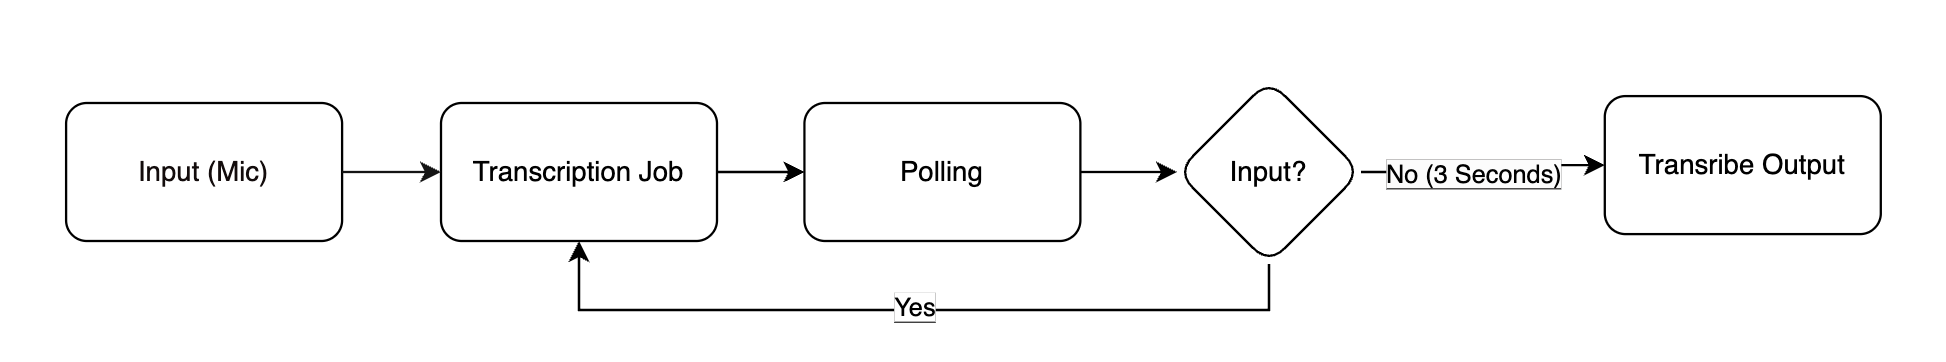
\includegraphics[width=\linewidth]{images/ASR_Pipeline.png}
    \caption{ASR pipeline using AssemblyAI}
    \label{fig: ASR_Pipeline.png}
\end{figure}

\subsubsection{Visual}
We decided to implements modular vision pipeline consisting of four sequential stages: object detection and segmentation, object classification, grasp synthesis, and scene understanding. Each stage is designed to progressively enrich the robot's understanding of its environments, with the ultimate goal of enabling reliable manipulation and task executive. \\

Our exploration has focused on leveraging foundation models such as the Segment Anything Model (SAM) for segmentation and CLIPs for classification, while ensuring modularity that allows integration with grasping algorithm (e.g., GraspNet) and higher-level reasoning (e.g. Vision-Language Models for scene understanding) ~\cite{segment-anything-2023,tlac-2025,hanwen2024_grasp,scene_seg}. \\

In this time period, we implemented and tested the first two stages of our vision pipeline: object segmentation and object classification \\


\textbf{Object Segmentation} \\


We used the SAM model to segment objects in tool-rich images. SAM successfully generated fine-grained masks and bounding boxes, producing over 50 detected regions per image as show in Figure ~\ref{fig: sam_pre}. 

\begin{figure}[H]
    \centering
    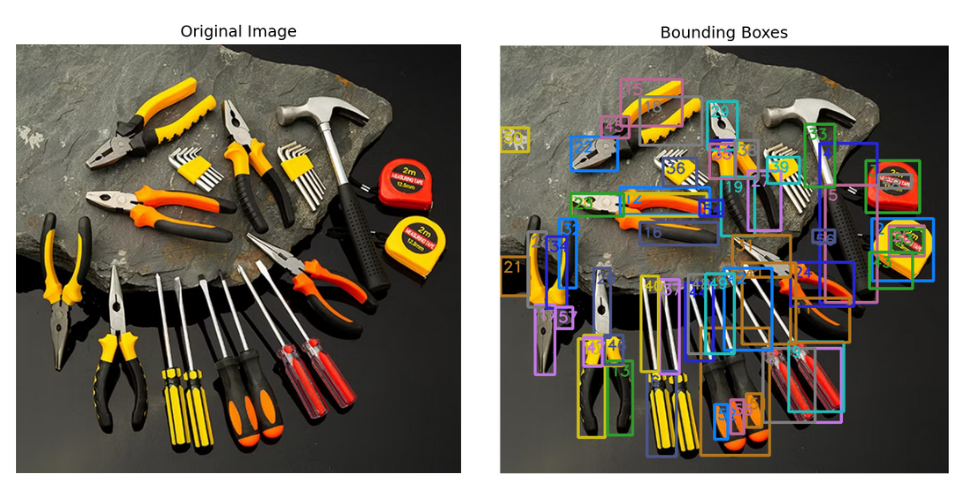
\includegraphics[width=\linewidth]{images/sam_pre.png}
    \caption{Segmentation results using the Segment Anything Model (SAM). 
    Elongated objects (e.g., pliers) are often over-segmented into multiple masks}
    \label{fig: sam_pre}
\end{figure}

However, elongated objects such as pliers were often split into multiple masks. To address this, we implemented a mask merging strategy based on bounding box overlap and mask adjacency. This reduced redundant detections and allowed us to consolidate fragmented masks into a single object representation.

\begin{figure}[htbp]
    \centering
    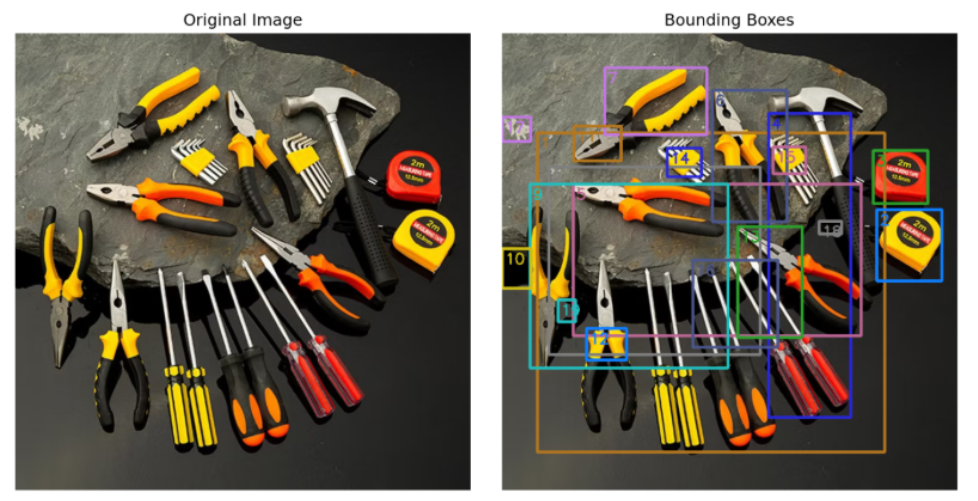
\includegraphics[width=\linewidth]{images/sam_post.png}
    \caption{Segmentation results after applying the mask merging strategy. 
    Over-segmented masks are combined into a unified representation}
    \label{fig: sam_post}
\end{figure}

\textbf{Object Classification} \\
We integrated CLIP embeddings with a curated tool embedding set covering 15 tool categories. After applying mask refinement, the cropped object regions fed into CLIP showed improved consistency. For example, screwdriver and pliers that were previously classified as multiple partial objects now produced stable predictions with higher confidence scores.

\begin{figure}[htbp]
    \centering
    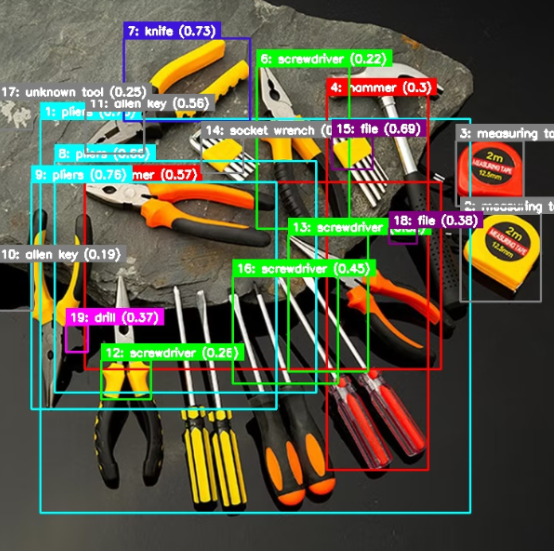
\includegraphics[width=0.5\linewidth]{images/clips_img.png}
    \caption{Object classification results using CLIP model}
    \label{fig: clips_img}
\end{figure}

By combining SAM segmentation with our refinement step and CLIP classification, we achieved more reliable object labeling across the dataset. Classification accuracy improved in terms of both stability (fewer duplicate predictions) and confidence values.

After implementing the segmentation and classification stages, we successfully completed the third and fourth stages of the vision pipeline: \textbf{grasp synthesis} and \textbf{scene understanding}. These modules mark a major step toward an end-to-end visual reasoning system capable of supporting robotic manipulation and navigation. \

\textbf{Grasp Synthesis} \
The grasp synthesis stage was implemented using the \textbf{GraspNet} framework~\cite{hanwen2024_grasp}, which predicts 6-DoF grasp configurations for segmented objects. As our depth camera has not yet arrived, we used curated RGB images from online sources combined with synthetic depth approximations to evaluate the performance of the complete perception pipeline. Each segmented region from SAM was converted into an object-centric point cloud and passed to GraspNet for grasp prediction. Despite the lack of real-world depth data, the synthesized pipeline demonstrated reliable grasp candidate generation, particularly for well-defined tools such as screwdrivers, hammers, and wrenches.

\begin{figure}[htbp]
\centering
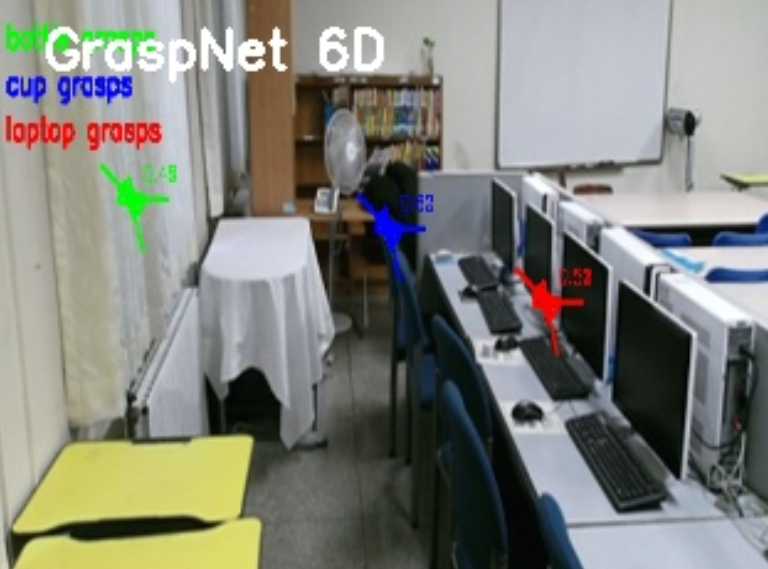
\includegraphics[width=0.5\linewidth]{images/graspnet_img.png}
\caption{Example of grasp synthesis results on internet-sourced RGB images. Predicted 6-DoF grasp poses are visualized with orientation markers.}
\label{fig: grasp_result}
\end{figure}


\begin{figure}[htbp]
\centering
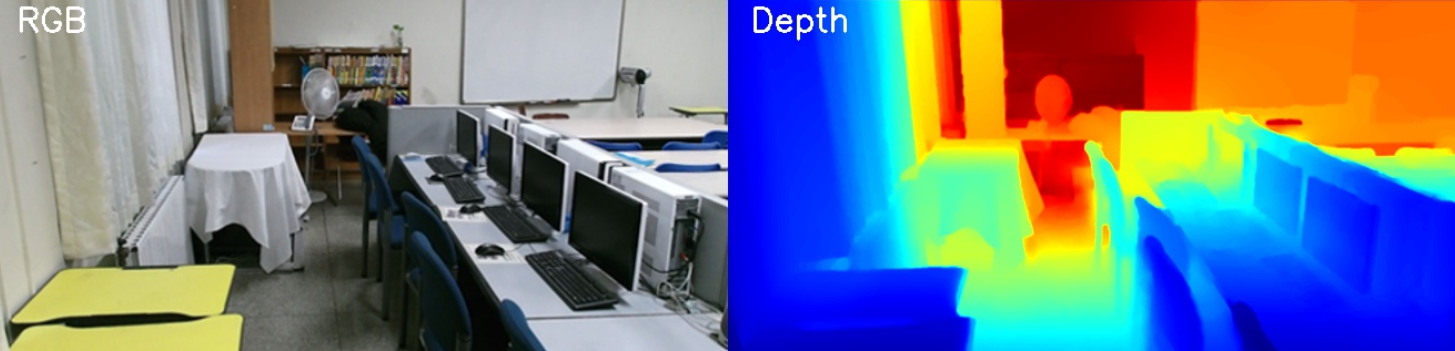
\includegraphics[width=\linewidth]{images/RGB-Dep.png}
\caption{A synthetic RGB-Depth image generated from an online RGB source using monocular depth estimation.}
\label{fig: grasp_result}
\end{figure}


\textbf{Scene Understanding} \
To extend the pipeline beyond individual object recognition, we implemented a scene understanding module that enables spatial reasoning between objects. By leveraging object centroids and bounding box coordinates derived from the segmentation and classification stages, the system can describe relative spatial relationships such as “the screwdriver is on the right of the pliers” or “the wrench is above the hammer.” This functionality was further enhanced using a lightweight Vision-Language Model (VLM) that supports contextual reasoning, allowing the robot to infer object grouping and hierarchical arrangements within a workspace.

\begin{figure}[htbp]
\centering
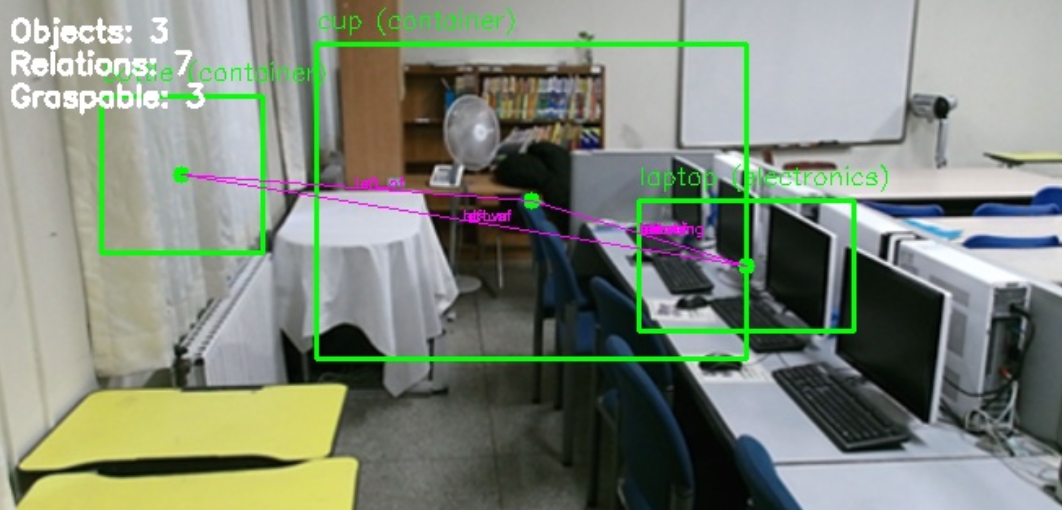
\includegraphics[width=0.5\linewidth]{images/scene_understanding.png}
\caption{Scene understanding results illustrating relative spatial relationships between detected tools.}
\label{fig: scene_understanding}
\end{figure}

To facilitate real-time interaction with robotic hardware, the completed perception pipeline—comprising SAM, CLIP, GraspNet, and Scene Understanding modules—was connected to a \textbf{ROS (Robot Operating System)} node. The pipeline publishes detection and grasping results as ROS topics, enabling seamless communication with motion planning and control modules. This setup establishes a modular framework that can be easily extended or replaced with higher-level planners.

\begin{figure}[htbp]
\centering
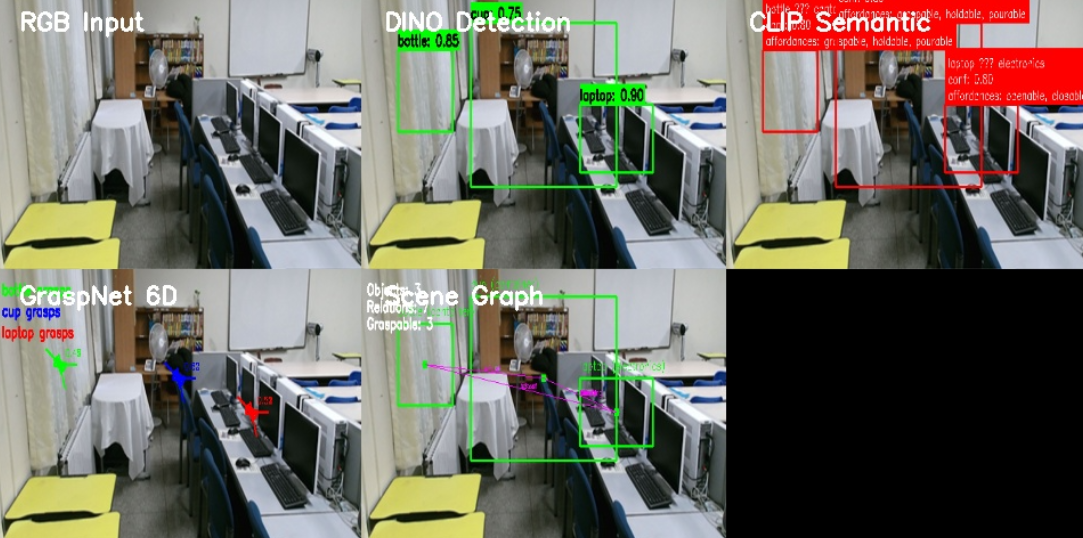
\includegraphics[width=\linewidth]{images/pipeline_image.png}
\caption{The complete vision pipeline from perception to reasoning. Demonstrating the progressive transformation of raw input data structured semantic and geometric understanding.}
\label{fig: grasp_result}
\end{figure}


In the upcoming phase, we will migrate the system to \textbf{ROS2} to enhance communication efficiency, scalability, and real-time performance across distributed nodes. Once the depth camera arrives, we will replace the synthetic image data with live RGB-D inputs to improve the accuracy of grasp synthesis and spatial reasoning. Additionally, we plan to refine image preprocessing and depth camera calibration to achieve higher visual accuracy, thereby simplifying path planning and manipulation tasks for the robot.


\subsubsection{Planning}

\begin{figure}[h]
    \centering
    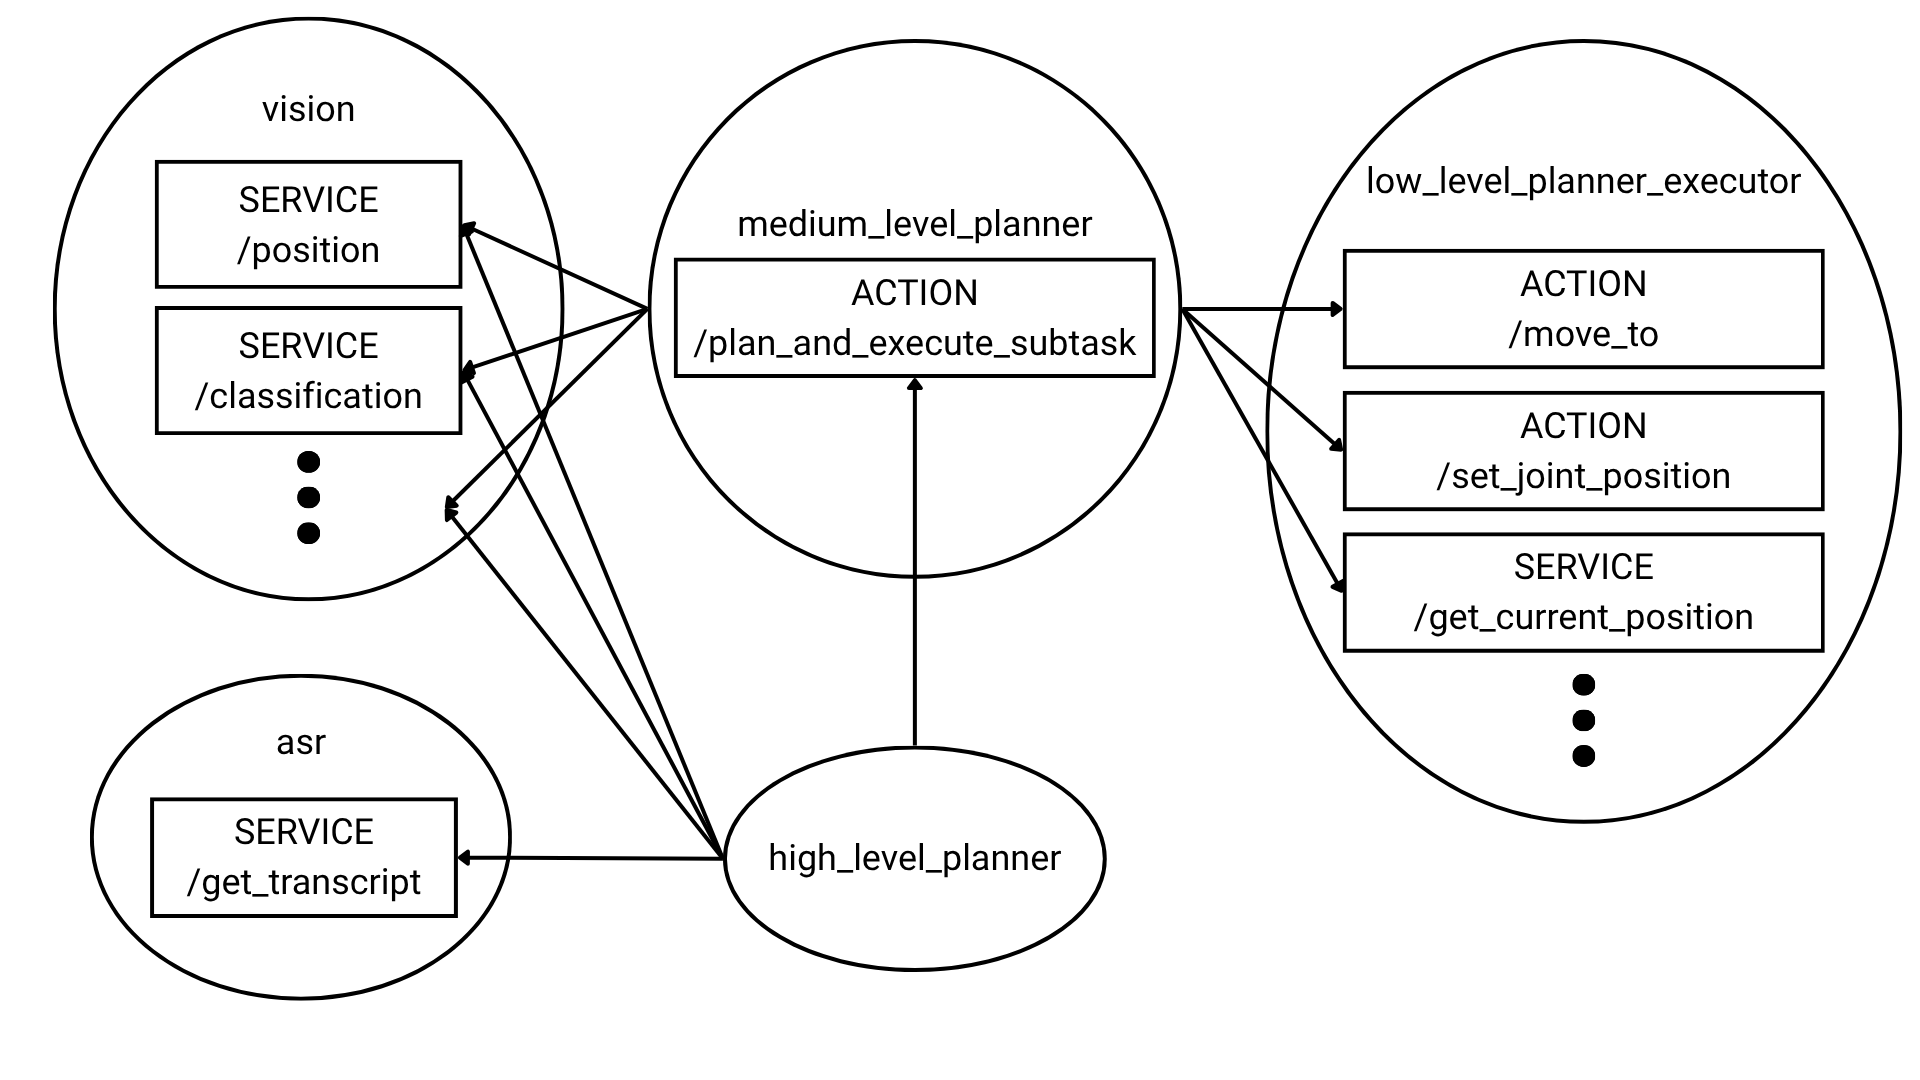
\includegraphics[width=\linewidth]{images/ros2_graph.png}
    \caption{High-level ROS2 Graph for Planning System}
    \label{fig: ros2-graph}
\end{figure}

Our current focus in planning is on low-level path planning and trajectory generation using MoveIt2~\cite{moveit2}, chosen for its strong integration with ROS2. We generated a MoveIt configuration package for the UR5e arm with the Robotiq 2F-85 gripper from our URDF using the MoveIt Setup Assistant.

Initial verification was done through the MoveIt2 GUI in RViz, confirming that inverse kinematics and trajectory planning worked correctly. We then extended control programmatically using the MoveIt2 C++ API by creating a ROS2 node, \texttt{moveit\_pose}, which hosts an action server \texttt{/plan\_execute\_pose}. This action takes a target end-effector pose and uses the \texttt{MoveGroupInterface} to plan and execute a trajectory from the current to the desired pose.

The planning pipeline is functional but not yet robust—plans occasionally fail or produce inefficient motions. To improve this, we are exploring tighter joint constraints, Cartesian path planning for smoother linear motion, and direct joint-space control through custom actions and services.

Beyond low-level motion planning, we have designed a hierarchical ROS2-based architecture consisting of five main nodes, as shown in Figure~\ref{fig: ros2-graph}, enabling modularity and extensibility across system layers:
\begin{enumerate}
    \item \textbf{vision:} Provides multiple perception-related services, including scene description, object classification, and object pose and position estimation.
    \item \textbf{asr:} Hosts the \texttt{/get\_transcript} service, which captures speech input, performs transcription, and returns the resulting text. Future improvements may include text-to-speech for enhanced interactivity.
    \item \textbf{high\_level\_planner:} Accesses all available services, receives high-level user instructions (via \texttt{/get\_transcript}), and decomposes them into structured subtasks.
    \item \textbf{medium\_level\_planner:} Implements an action server to plan and execute these subtasks by converting them into “robot language” consisting of via-points and gripper actions.
    \item \textbf{low\_level\_planner\_executor:} Handles path planning, trajectory generation, inverse kinematics, and motion execution, exposing corresponding services and action servers.
\end{enumerate}

This multi-layered design allows each component to be developed, replaced, or improved independently. The hierarchical decomposition of planning—from perception and language understanding down to motion execution—enables the robot to perform complex, long-horizon tasks while maintaining system modularity and flexibility.



\subsubsection{Simulation}

\begin{figure}[h]
    \centering
    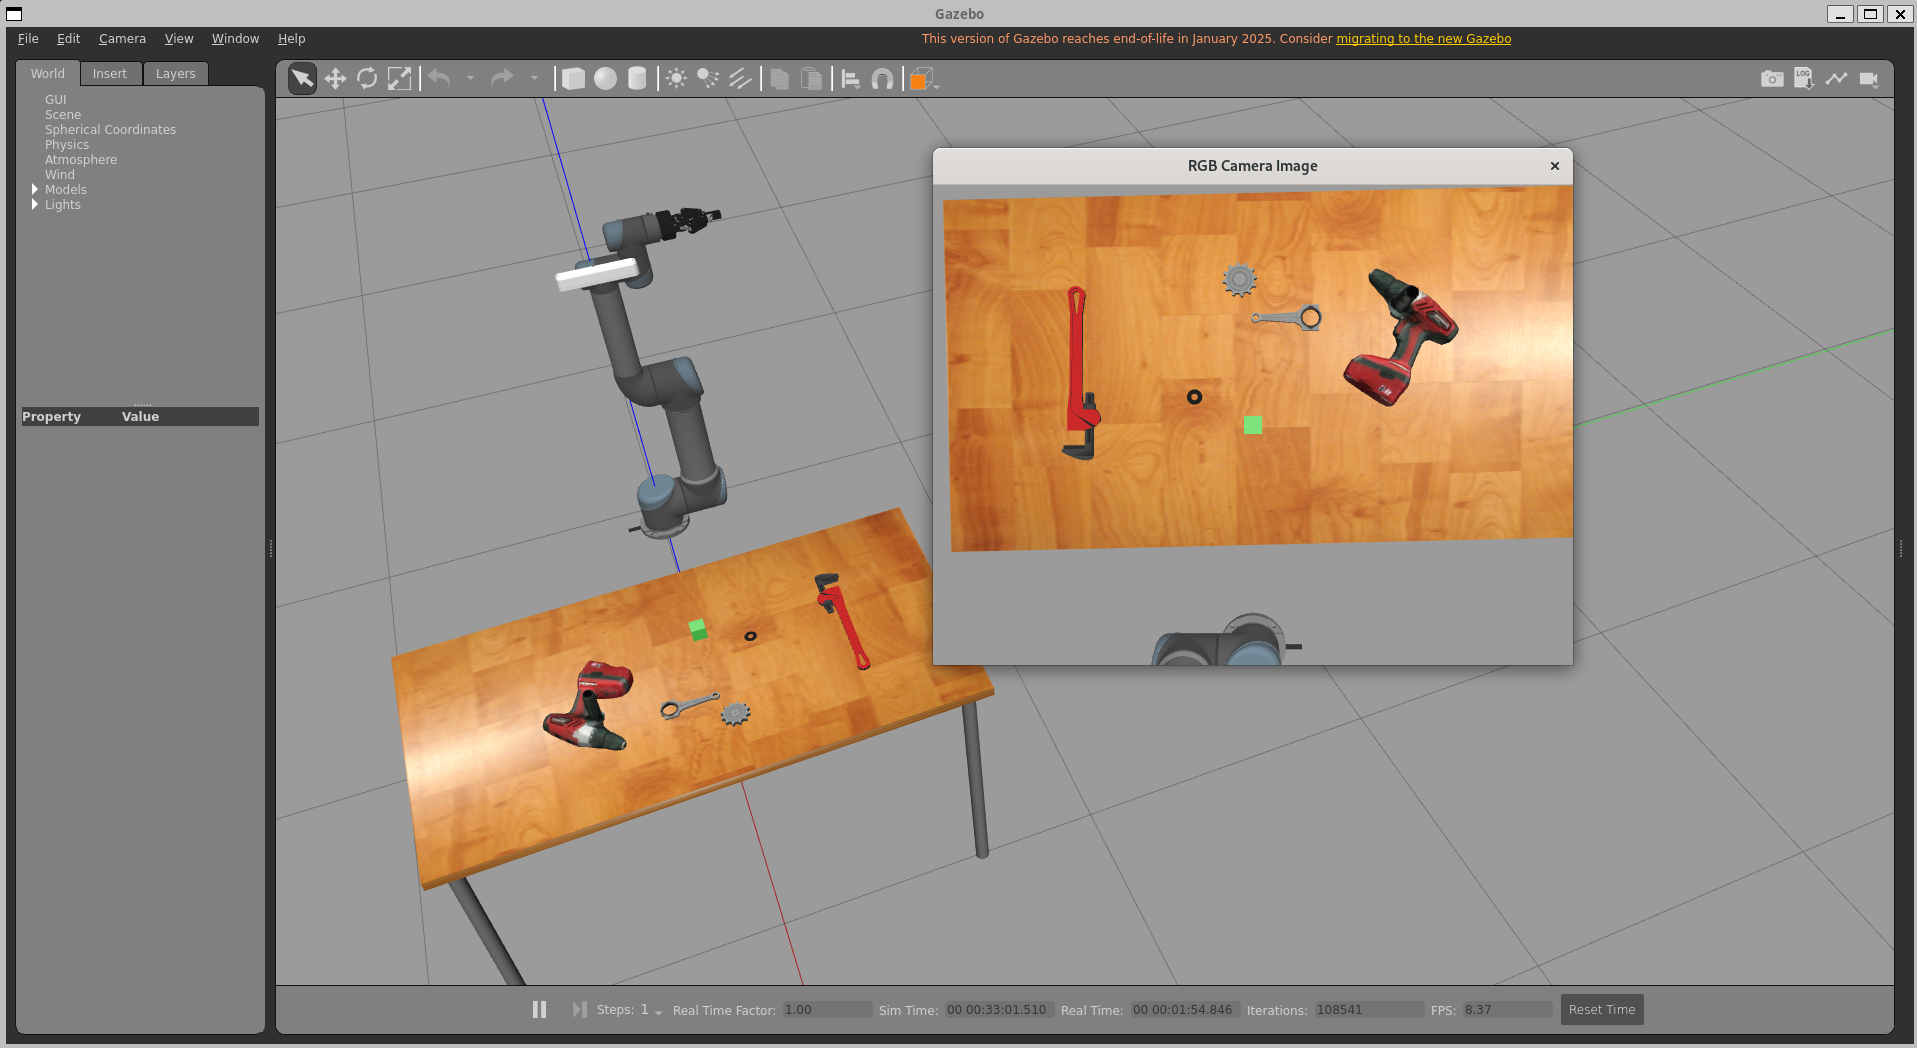
\includegraphics[width=\linewidth]{images/gazebo_setup.png}
    \caption{UR5 with Robotiq 2F-85 gripper and depth camera in Gazebo simulation environment}
    \label{fig: gazebo-setup}
\end{figure}

\begin{figure}[h]
    \centering
    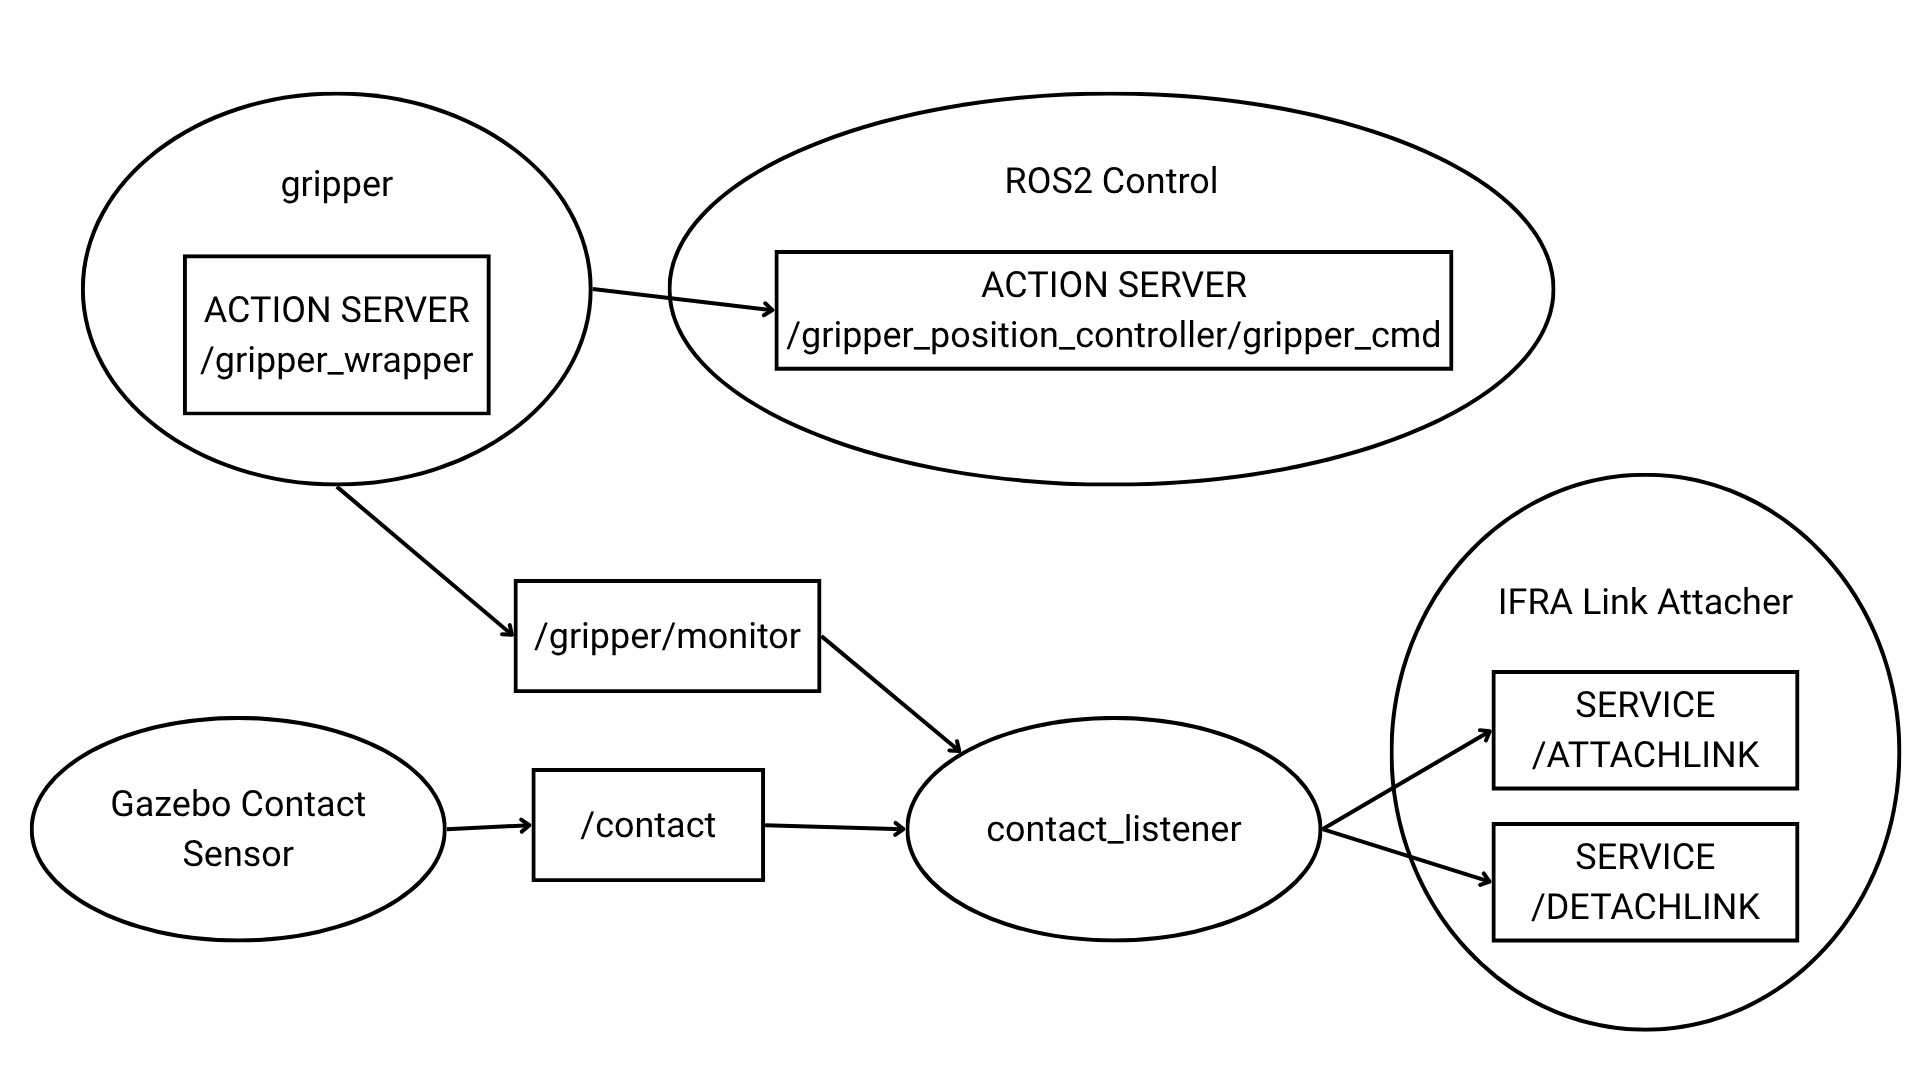
\includegraphics[width=\linewidth]{images/ros2_sim_graph.png}
    \caption{ROS2 Graph for Gazebo Simulation Setup}
    \label{fig: ros2-sim-graph}
\end{figure}

Our simulation initially began in Isaac Sim, where we verified ROS2 integration, motion planning with MoveIt2, and perception-enabled obstacle avoidance using a UR5 robot, Robotiq 2F-85 gripper, and Intel RealSense D435i camera. However, Isaac Sim’s limitations in handling closed-loop mechanisms prevented proper gripper motion, making it complex and difficult to simulate pick-and-place tasks.

We therefore transitioned to Gazebo Classic, chosen over Gazebo Ignition (now \textit{Gazebo}) for plugin compatibility. The environment includes the UR5, Robotiq gripper, a table, and a downward-facing camera, as shown in Figure~\ref{fig: gazebo-setup}. ROS2 communication between the robot, gripper, and sensors is verified through standard Gazebo ROS2 interfaces.

To address the challenge of simulating object grasping, we use the IFRA Link Attacher Plugin~\cite{ifra_link_attacher}, which provides the \texttt{/ATTACHLINK} and \texttt{/DETACHLINK} services to dynamically create or destroy fixed joints between links—effectively simulating gripping and releasing actions. A Gazebo contact sensor is mounted on the gripper finger link to detect collisions. Since contact data is only published internally within Gazebo, we implemented a custom plugin that forwards this data to a ROS2 topic \texttt{/contact}. A ROS2 node, \texttt{contact\_listener}, subscribes to this topic and calls \texttt{/ATTACHLINK} when contact with an object is detected.

For releasing, we control the gripper via the ROS2 action\\\texttt{/gripper\_position\_controller/gripper\_cmd}\\. A wrapper node, \texttt{gripper}, exposing \texttt{gripper\_wrapper} action, forwards these commands while also publishing their status to \texttt{/gripper/monitor}. The \texttt{contact\_listener} subscribes to this topic and, when detecting that the gripper is opening, calls \texttt{/DETACHLINK} if any attachments exist. This combination enables dynamic, automated grasping and releasing behavior. A diagram of all ROS2 elements is shown in Figure~\ref{fig: ros2-sim-graph}.

We also integrated our vision pipeline using the cv\_bridge~\cite{cv_bridge} package to convert Gazebo image messages into OpenCV-compatible formats. The simulation world includes models of engineering tools and parts for vision testing. However, many models have simplified collision geometries, which makes gripping small or slender parts difficult. Our advisor has advised us to use the simulation for the path planning and trajectory generation, while the grasping will be tested on the real robot.

In summary, the Gazebo Classic environment now provides a complete simulation of perception, planning, and dynamic grasping, forming a robust foundation for testing our integrated robotic system.

\subsubsection{Hardware}

\begin{figure}[h]
\centering
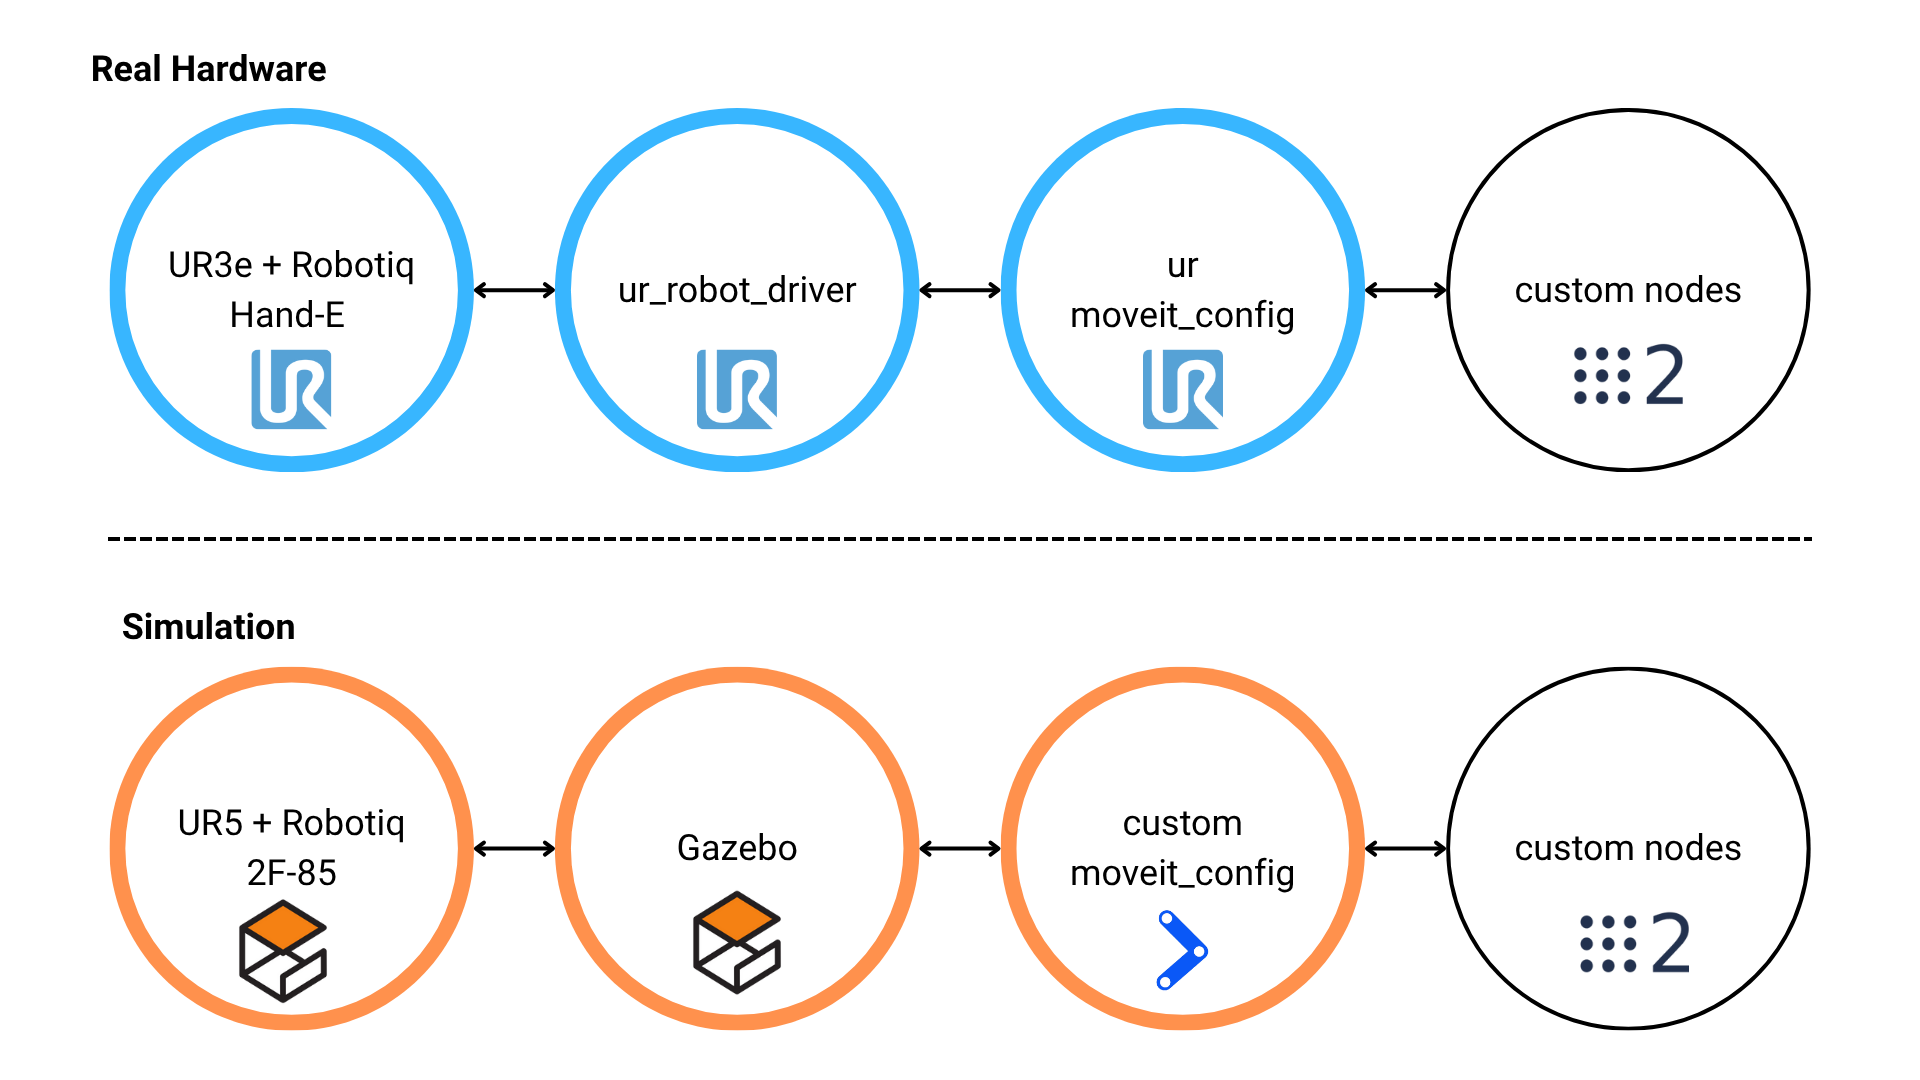
\includegraphics[width=\linewidth]{images/sim_vs_real.png}
\caption{Comparison between Simulation (Gazebo) and Real Hardware Setup (UR3e with Robotiq HandE gripper at Chulapat 14 Robotics Lab)}
\label{fig: sim-vs-real}
\end{figure}

For connecting with the real hardware, we first set up a dual-boot environment on our computer to run Ubuntu 22.04 natively, instead of using the previous Windows Subsystem for Linux (WSL) configuration. This change significantly reduces network complexity and communication latency between the computer and the UR arm, ensuring smoother and more reliable control.

We use the official Universal Robots ROS2 Driver~\cite{ur_ros2_driver}, which directly interfaces with the UR arm and replaces Gazebo in our simulation setup. The driver provides a standardized ROS2 interface to the physical robot and comes with the \texttt{ur\_moveit\_config} package, enabling us to use MoveIt2 for path planning, trajectory generation, and motion execution on the real UR arm.

Our setup uses the UR3e robot equipped with a Robotiq HandE gripper located at the Chulapat 14 Robotics Lab. The UR3e already includes the necessary software to support ROS2 communication through the External Control URCap. We connect our computer to the UR control box via a dedicated Ethernet cable and configure the computer’s network interface to the IP address \texttt{10.10.0.5}, as expected by the robot. Once the connection is established, we launch the External Control program on the robot’s teach pendant and verify successful communication by commanding robot motions through the ROS2 driver and MoveIt2 interface.

To ensure seamless interoperability between simulation and hardware, we modified our existing node to support both environments. The changes include dynamically adjusting the MoveIt2 move group name and toggling the \texttt{use\_sim\_time} parameter depending on whether the system is operating in Gazebo or on the real robot. We verified that the same service and action calls produced identical behavior in both the simulation and the real hardware environment, confirming consistent motion planning and execution across both setups.

\newpage
\section{Project Planning}
The project is structured around four primary technical area of concentration exluding any relevant paperwork tasks. These align seamlessly with the core enhancements, which will all be implemented in parallel: \textbf{image processing, speech processing, planning algorithms, and robotic arm integration}.  The planned timeline is structured into weekly milestones to ensure iterative progress and early validation 

\begin{figure}[htbp]
    \centering
    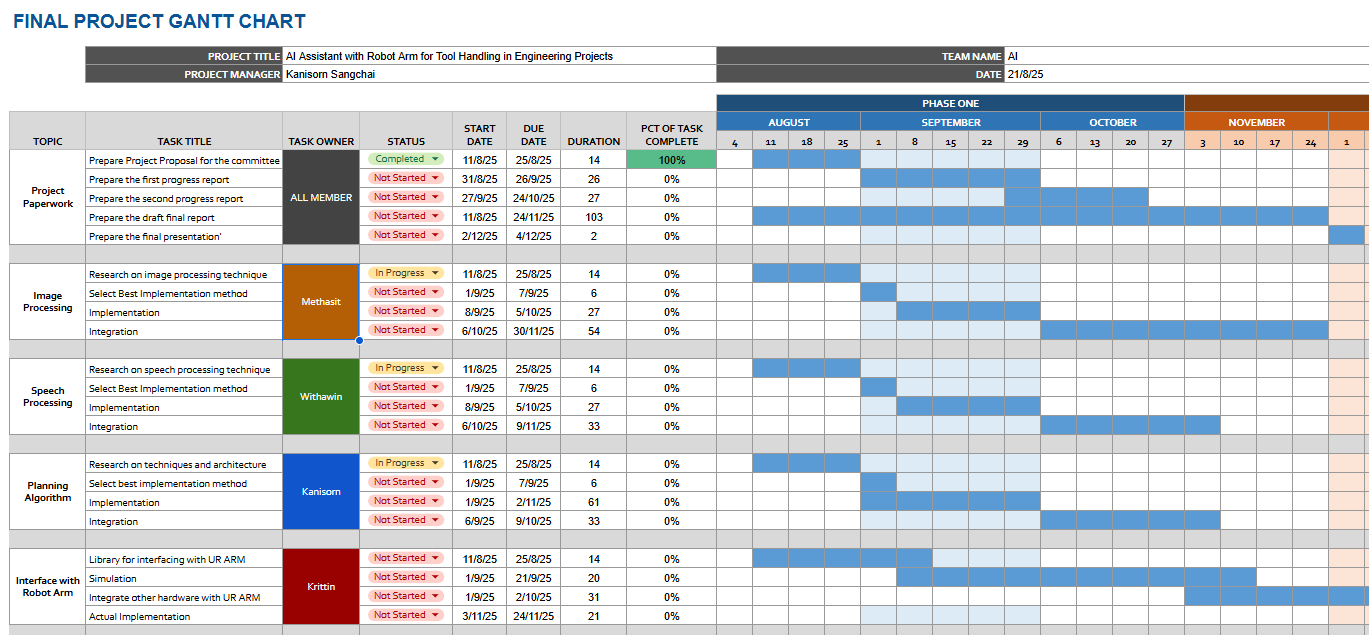
\includegraphics[width=0.8\linewidth]{images/Gantt_chart(2).png}
    \caption{A proposed project timeline scheduled for the project’s implementation in this semester}
    \label{fig:gantt-chart}
\end{figure}

\subsection{Initial Timeline}

\subsubsection{Image Processing}
[2 Weeks] Research on image processing techniques 
\begin{itemize}
    \item A literature review and exploration of existing approaches will be conducted to identify suitable image processing methods for robotic applications.
\end{itemize}
[1 Week] Select best implementation method
\begin{itemize}
    \item Based on the research findings, the team will decide on the most promising method to pursue further development.
\end{itemize}
[4 Weeks] Implementation
\begin{itemize}
    \item The chosen method will be implemented, with iterative testing to verify accuracy, robustness, and suitability for integration with the robot system.
\end{itemize}
[8 Weeks] Integration
\begin{itemize}
    \item The implemented solution will be connected to the overall system, ensuring compatibility and real-time performance with the robotic platform.
\end{itemize}
\subsubsection{Speech Processing}
[3 Weeks] Research on speech processing techniques
\begin{itemize}
    \item A comprehensive study on speech-to-command systems will be carried out to identify feasible methods for tool-handling tasks.
\end{itemize}
[1 Week] Select best implementation method
\begin{itemize}
    \item The most effective speech processing model or framework will be selected after evaluating feasibility, latency, and accuracy.
\end{itemize}
[5 Weeks] Implementation
\begin{itemize}
    \item The selected method will be developed into a working module, with error handling and adaptability to diverse inputs.
\end{itemize}
[5 Weeks] Integration
\begin{itemize}
    \item The module will be integrated into the robot system to ensure smooth operation, including communication between the speech module and task-planning system.
\end{itemize}
\subsubsection{Planning Algorithm}
[3 Weeks] Research on techniques and architectures
\begin{itemize}
    \item A review of different approaches and existing planning algorithms will be conducted to identify suitable architectures.
\end{itemize}
[1 Weeks] Select best implementation method
\begin{itemize}
    \item Candidate techniques will be compared, and the optimal method will be chosen for development.
\end{itemize}
[5 Weeks] Implementation
\begin{itemize}
    \item The selected approach will be implemented with an emphasis on ensuring symbolic reasoning and adaptability to real-world tasks.
\end{itemize}
[5 Weeks] Integration
\begin{itemize}
    \item The algorithm will be integrated into the system to handle planning tasks, translating perception (image/speech) into robotic execution commands.
\end{itemize}
\subsubsection{Interface with Robot Arm}
[5 Weeks] Develop library for interfacing with UR Arm
\begin{itemize}
    \item A dedicated library will be created to enable seamless communication with the UR robotic arm.
\end{itemize}
[10 Weeks] Simulation
\begin{itemize}
    \item Virtual simulations will be performed to verify system stability and safety before real-world trials.
\end{itemize}
[5 Weeks] Integrate other hardware with UR Arm
\begin{itemize}
    \item Additional supporting hardware will be tested and interfaced to ensure full robotic tool-handling capabilities.
\end{itemize}
[2\textsuperscript{nd} semester] Actual implementation
\begin{itemize}
    \item The final robotic interface will be tested and deployed on the physical UR Arm, completing the integration.
\end{itemize}

\subsection{Current Timeline}

\subsubsection{Image Processing}

The development of the image processing module is proceeding on schedule and has entered the system integration phase. Core functionalities, including image acquisition, preprocessing, segmentation, and scene understanding have been successfully implemented and validated through controlled experiments. The development has now entered the integration phase, focusing on seamless communication with the overall robotic framework. Ongoing work involves synchronizing image data streams with the motion planning and control modules to enable end-to-end perception-driven operation.

\subsubsection{Speech Processing}

The development of the Automatic Speech Recognition (ASR) module is proceeding on schedule and has entered the system integration phase. Core functionalities, including live audio capture, real-time transcription, silence detection, and ROS2 publishing, have been successfully implemented and validated through controlled tests. The development has now entered the integration phase, focusing on seamless communication with the \textbf{real-world UR-ARM}. Ongoing work involves integrating the ASR outputs with the robot's control modules to enable end-to-end speech-driven manipulation.

\subsubsection{Planning Algorithm}
The current progress is on schedule, with low-level motion planning and execution successfully implemented and verified through simulation and programmatic control. The system can now autonomously plan and execute trajectories, though ongoing refinements aim to improve reliability and efficiency. Development is advancing toward high-level planning and integration with the perception module within a hierarchical, modular architecture that enables coordinated, extensible, and intelligent robot behavior across all system layers.

\subsubsection{Interface with Robot Arm}
The simulation environment has been fully developed and is now ready for integration with perception and planning modules. Dynamic grasping enables end-to-end testing of the robotic system. Initial challenges with gripper motion led to a transition to a more compatible setup, where object interaction and motion execution now function reliably. The current progress is on schedule, with the simulation serving as a robust platform for validating motion planning and perception integration before transferring grasping tests to the real hardware.

\newpage
\section{Theory and Technical Backup}

\subsection{Voice Control Systems (VCS)}
Voice control systems have significantly transformed human-computer interaction by enabling users to interact with interfaces using voice commands and natural language. These systems leverage automatic speech recognition (ASR) to convert voice recordings into text, and advancements in deep learning have greatly enhanced their capabilities, alongside natural language processing. VCS offers numerous benefits, including saving users time and resources by providing quick services through an efficient interface without requiring extensive additional devices. They foster natural voice communication between users and devices, enhancing user comfort and creating a more intuitive interface. The adoption rate of voice-activated digital assistants has increased substantially, leading to a wide array of Internet of Things (IoT) devices incorporating voice-activated user interfaces for tasks ranging from creating grocery lists to controlling smart homes. Beyond smart gadgets and IoT, VCS technology is also applied in automotive systems to prevent accidents by allowing drivers to focus on their surroundings. VCS significantly improves the quality of life for various groups, including elderly people, children under four, and individuals with physical disabilities. They can provide complete control over home or office appliances, facilitate traffic regulation, and enhance healthcare systems~\cite{vcs}.

\subsection{Multimodal Automatic Speech Recognition}

\begin{figure}[htbp]
    \centering
    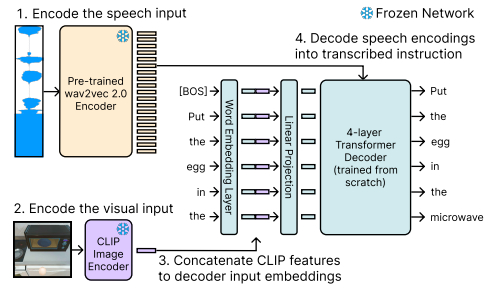
\includegraphics[width=0.8\linewidth]{asr}
    \caption{Multimodal ASR model architecture.
    (from~\cite{Chang2023})}
    \label{fig:asr}
\end{figure}

Multimodal Automatic Speech Recognition (ASR) enhances speech transcription by integrating visual context alongside audio signals, which is crucial for tasks such as embodied agents and human-robot interaction. By leveraging both modalities, multimodal ASR improves robustness and accuracy over traditional unimodal systems, achieving lower Word Error Rate (WER) and higher Recovery Rate (RR), especially under noisy or masked audio conditions. It is particularly effective at recovering visually salient words, such as object names, thereby increasing task completion rates in instruction-following scenarios~\cite{Chang2023},\cite{multi}.

Typical architectures combine a speech encoder, such as wav2vec 2.0, with a visual encoder, often based on CLIP-ViT, feeding both into a Transformer-based decoder that attends jointly to audio and visual features. Unlike unimodal ASR, which relies only on speech input, multimodal ASR grounds transcription in environmental context, reducing ambiguity and improving generalization to unseen speakers and settings~\cite{Chang2023},\cite{multi}.

Applications include benchmarks like ALFRED, where agents must interpret spoken instructions to navigate and manipulate objects, as well as real-world human-robot communication. Compared with unimodal baselines, multimodal ASR achieves superior masked word recovery (up to 30\% more) and mitigates performance degradation in noisy conditions~\cite{Chang2023},\cite{multi}. Challenges remain regarding generalization to real-world environments, as many studies rely on synthetic data and simplified noise models.

\subsection{Neuro-Symbolic Artificial Intelligence (NSAI)}

\begin{figure}[htbp]
    \centering
    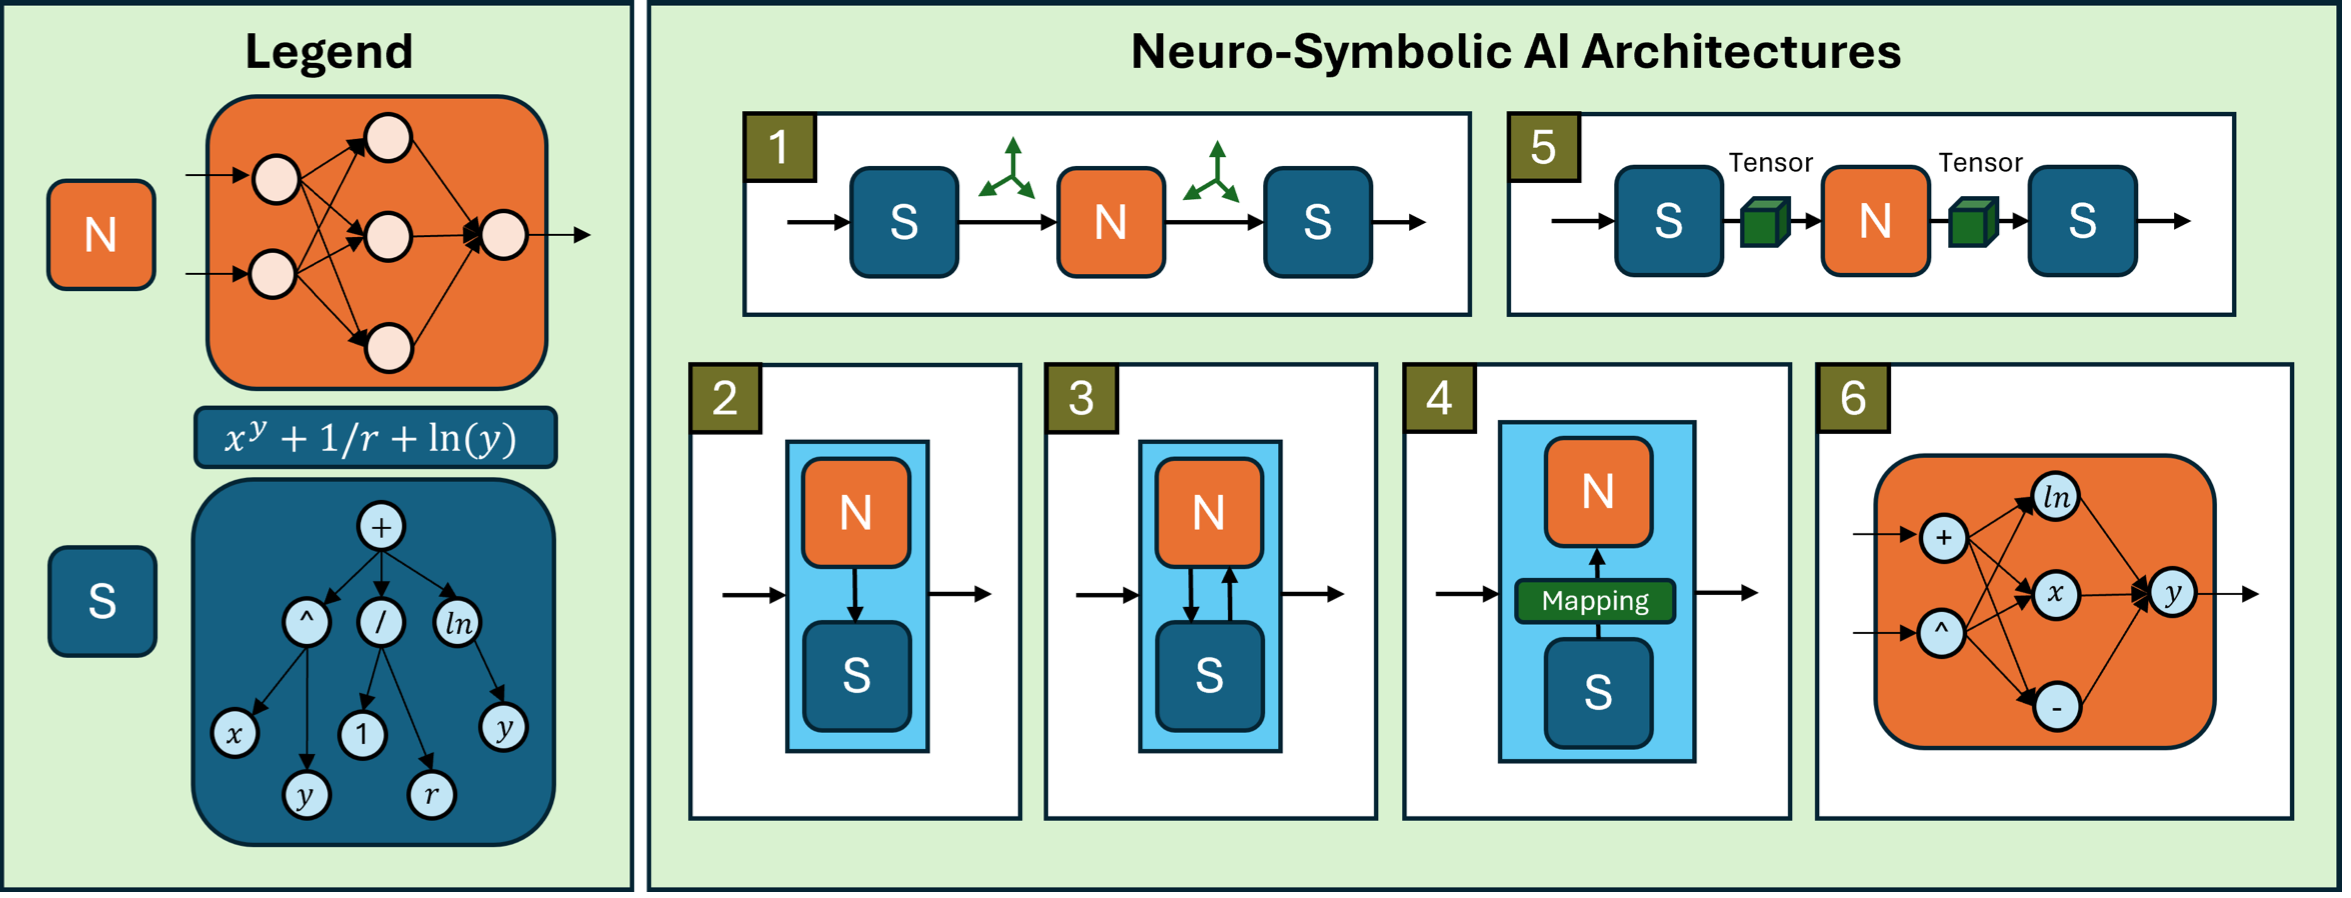
\includegraphics[width=0.8\linewidth]{nsai-types}
    \caption{Neuro-Symbolic AI types
    (from~\cite{nsai})}
    \label{fig:nsai-types}
\end{figure}

Neuro-Symbolic Artificial Intelligence (NSAI) is an emerging paradigm that combines the strengths of neural networks with symbolic reasoning. Neural networks excel in pattern recognition and data-driven learning but often lack explainability and explicit reasoning capabilities, operating as "black boxes". In contrast, symbolic AI is inherently interpretable and excels in logical reasoning but struggles with perception from raw data and requires extensive manual knowledge engineering. NSAI aims to bridge these gaps by integrating the robust statistical learning of neural networks with the structured knowledge and logic of symbolic AI, enabling systems to reason, make decisions, and generalize knowledge more effectively from large datasets. This hybrid approach enhances interpretability, robustness, and trustworthiness, while also facilitating learning from less data~\cite{nsai}.\\
NSAI systems can be categorized into various architectures based on the connection between their neural and symbolic components, as shown in Figure~\ref{fig:nsai-types}. These include:
\begin{itemize}

    \item \textbf{Symbolic Wrapper (Type 1)}: Symbolic systems guide both input and output, leveraging neural networks internally for data-driven learning (e.g., DeepProbLog, Neuro-Symbolic Concept Learner (NSCL), hybrid neuro-symbolic robotics).

    \item \textbf{Symbolic [Neuro] (Type 2)}: Symbolic systems dominate, with neural modules used internally for perception and pattern recognition (e.g., in autonomous communication or scene interpretation).

    \item \textbf{Bidirectional Interaction (Type 3)}: Neural and symbolic components tightly interact, with neural models adjusting outputs based on symbolic constraints and symbolic modules evolving reasoning based on neural feedback (e.g., AlphaGo, AlphaZero, in robotics).

    \item \textbf{Sequential Connection (Type 4)}: Neural networks connect sequentially to symbolic systems via an explicit mapping layer, converting continuous neural outputs into structured symbolic knowledge (e.g., Neural Symbolic Machines (NSM)).

    \item \textbf{Embedded Symbolic Information (Type 5)}: Symbolic information is directly embedded into tensor representations, enhancing neural network reasoning in a differentiable manner (e.g., Logic Tensor Networks (LTNs)).

    \item \textbf{Deeply Integrated (Type 6)}: Symbolic structures are directly processed by neural networks, blending symbolic reasoning and neural computation seamlessly (e.g., Neural Theorem Provers (NTP), Graph Neural Networks (GNNs)).
\end{itemize}

\subsection{Large Language Model (LLM)}

\begin{figure}[htbp]
    \centering
    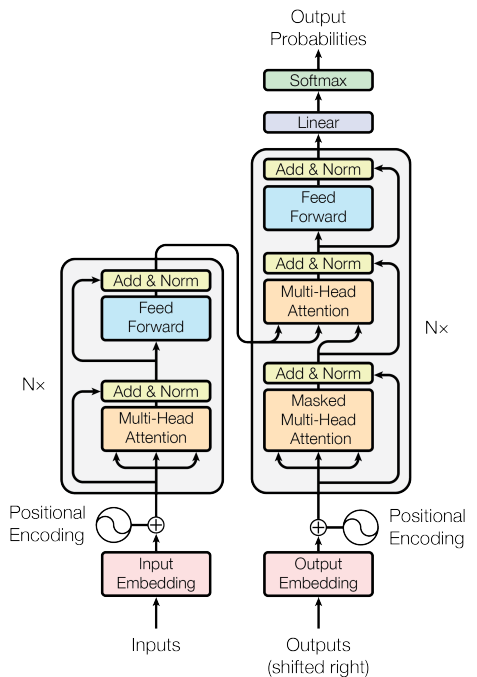
\includegraphics[width=0.5\linewidth]{transformer}
    \caption{The Transformer-model architecture
    (from~\cite{attention-is-all-you-need})}
    \label{fig:transformer}
\end{figure}

Large Language Models (LLMs), such as BERT and GPT-5, are pretrained neural networks that serve as powerful foundation models for language understanding and generation. They build on the Transformer architecture, shown in Figure~\ref{fig:transformer}, a sequence model that relies entirely on attention mechanisms and avoids recurrence or convolutions. The Transformer employs an encoder-decoder structure with stacked layers of multi-head self-attention and feed-forward networks, enabling the model to relate different positions within a sequence and capture diverse representation subspaces. Positional encodings are added to input embeddings to provide information about token order~\cite{attention-is-all-you-need}. LLMs represent words as vectors and acquire robust language and world knowledge through large-scale self-supervised learning, such as predicting masked words or the next word in a sequence. These models excel at tasks including machine translation, question answering, text classification, and text generation, leveraging vast amounts of text data to learn meanings and factual knowledge. Despite their capabilities, LLMs have limitations in deep understanding, reasoning, and completeness of knowledge, and raise societal concerns regarding bias and centralized model control~\cite{human-language-understanding}.

The reason why it is preferred over traditional Natural Language Processing (NLP) models is due to
the impressive ability to grasp broad contexts with little to no training. Mostly outperforms various
Natural Language Processing (NLP) techniques without having to fine-tune with execution cost.
Among the algorithms capable of handling a range of Natural Language Processing tasks, Large
Language Model (LLM) has not only frequently appeared in numerous past studies but has also
showcased immense potential for generating plans, transforming an initial world state into a desired state~\cite{plangenllm}.

\subsection{Vision Language Model (VLM)}
\begin{figure}[htbp]
    \centering
    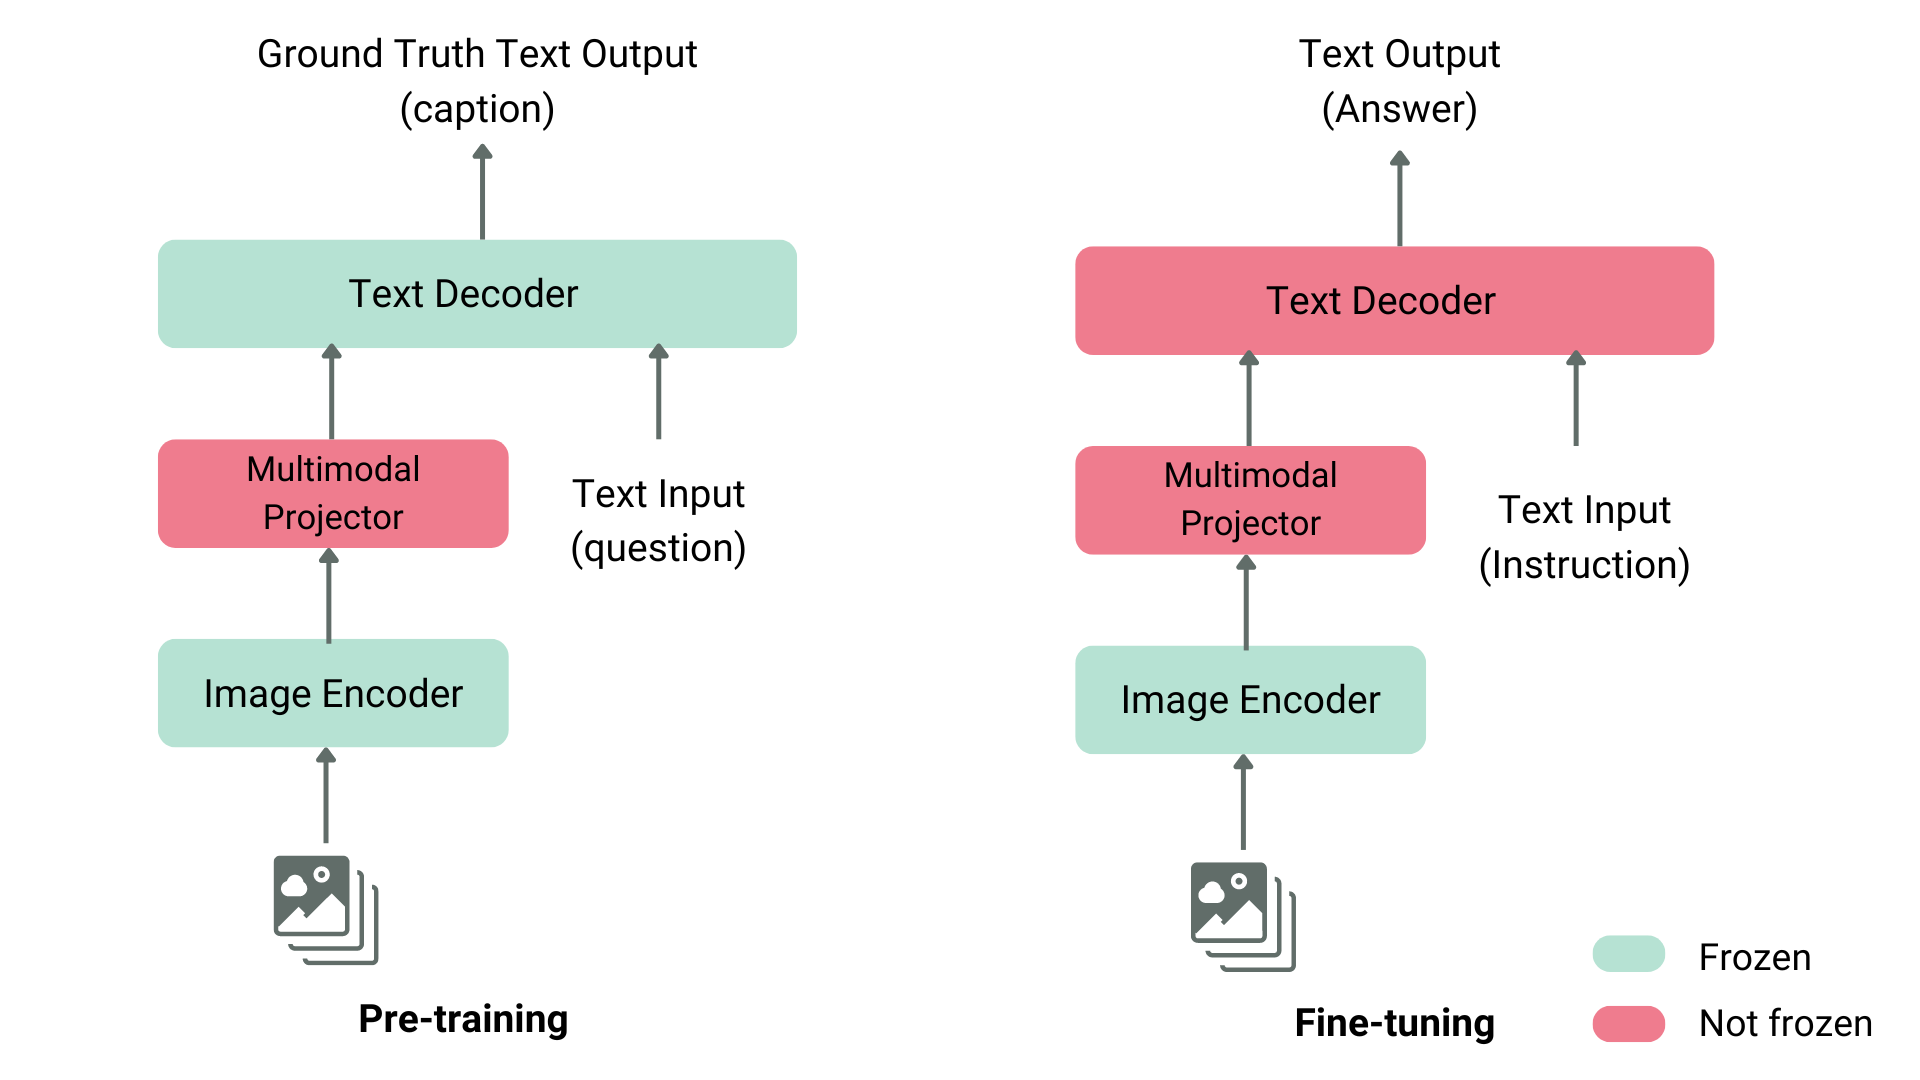
\includegraphics[width=0.8\linewidth]{images/vlm-structure.png}
    \caption{Structure of a Typical Vision Language Model (from~\cite{huggingface_vlms_2024})}
    \label{fig:vlm-structure}
\end{figure}

Vision Language Models (VLMs) are multimodal generative AI models that combine image and text understanding to perform a wide range of tasks, including visual question answering, image captioning, document analysis, and instruction-based image recognition. Many VLMs can also reason about spatial relationships in images, producing outputs like bounding boxes or segmentation masks. Architecturally, they usually consist of an image encoder, a projection layer that aligns image and text embeddings, and a text decoder for generating output, as shown in Figure~\ref{fig:vlm-structure}. Popular open-source VLMs include LLaVA, KOSMOS-2, Qwen-VL, CogVLM, and Fuyu-8B, each varying in model size, supported features such as chat or grounding, and image resolution~\cite{huggingface_vlms_2024}.

VLMs are powerful in zero-shot generalization, allowing them to handle unseen images and prompts without additional training. Furthermore, fine-tuning allows adaptation to specialized applications, such as educational tools, interactive assistants, or automated document evaluation. Their limitations include susceptibility to hallucinations, biases from training data, and high computational requirements for end-to-end training or large models~\cite{huggingface_vlms_2024}.
\subsection{Vision-Language-Action (VLA) Models}

\begin{figure}[htbp]
    \centering
    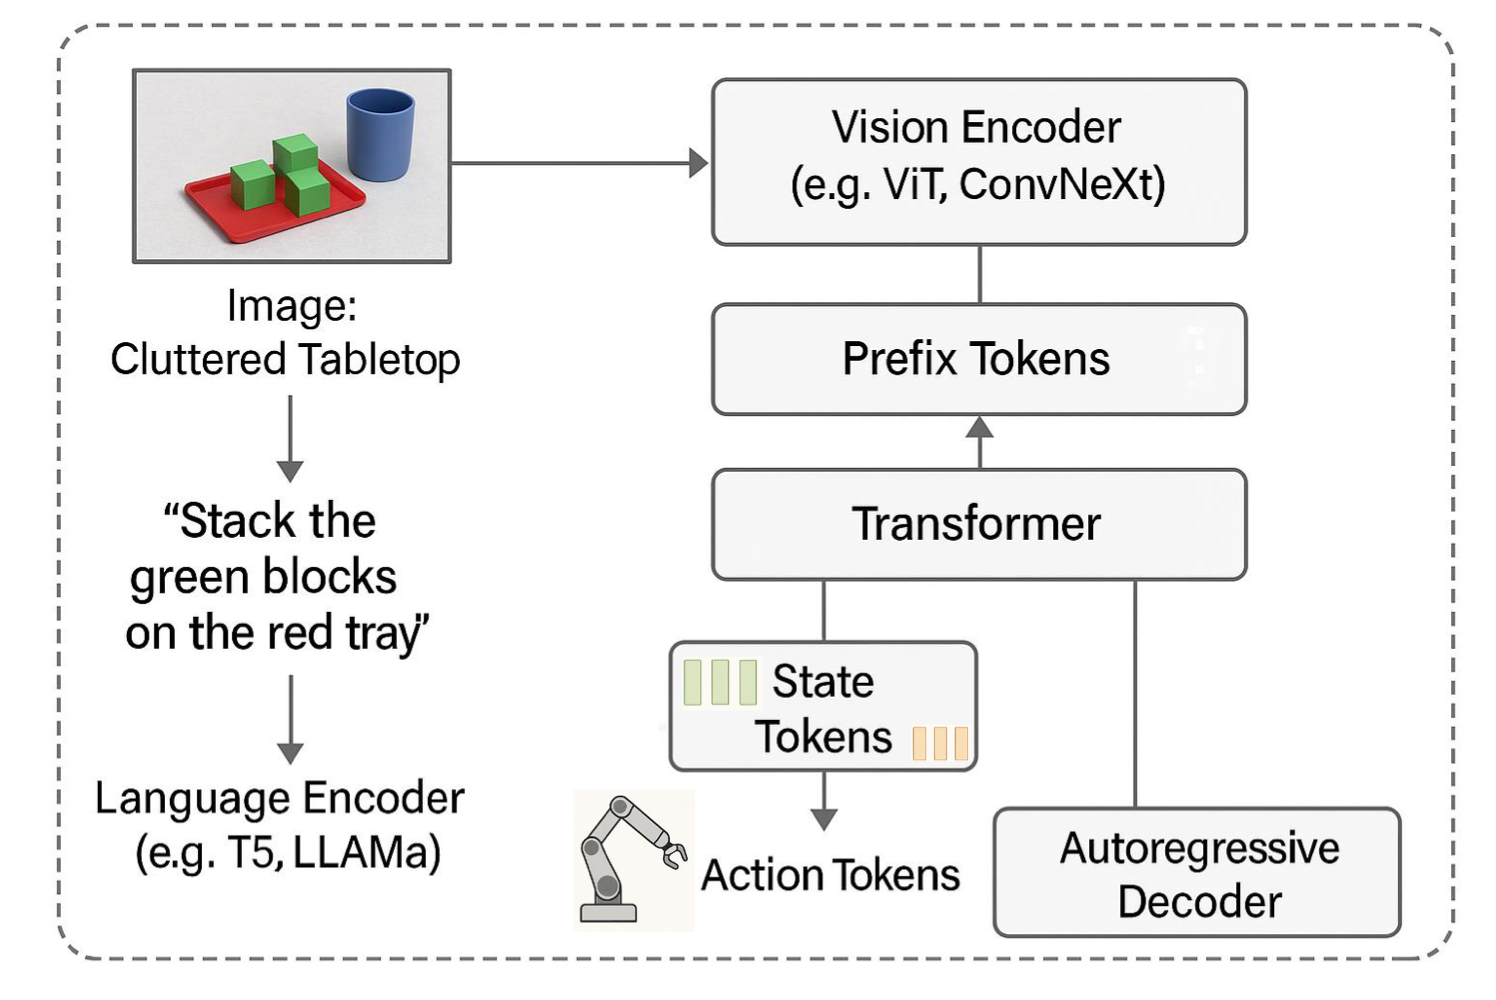
\includegraphics[width=0.8\linewidth]{images/vla.png}
    \caption{End-to-end Tokenization and Representation Process in VLA Models (from~\cite{vla})}
    \label{fig:vla}
\end{figure}

\begin{figure}[h]
    \centering
    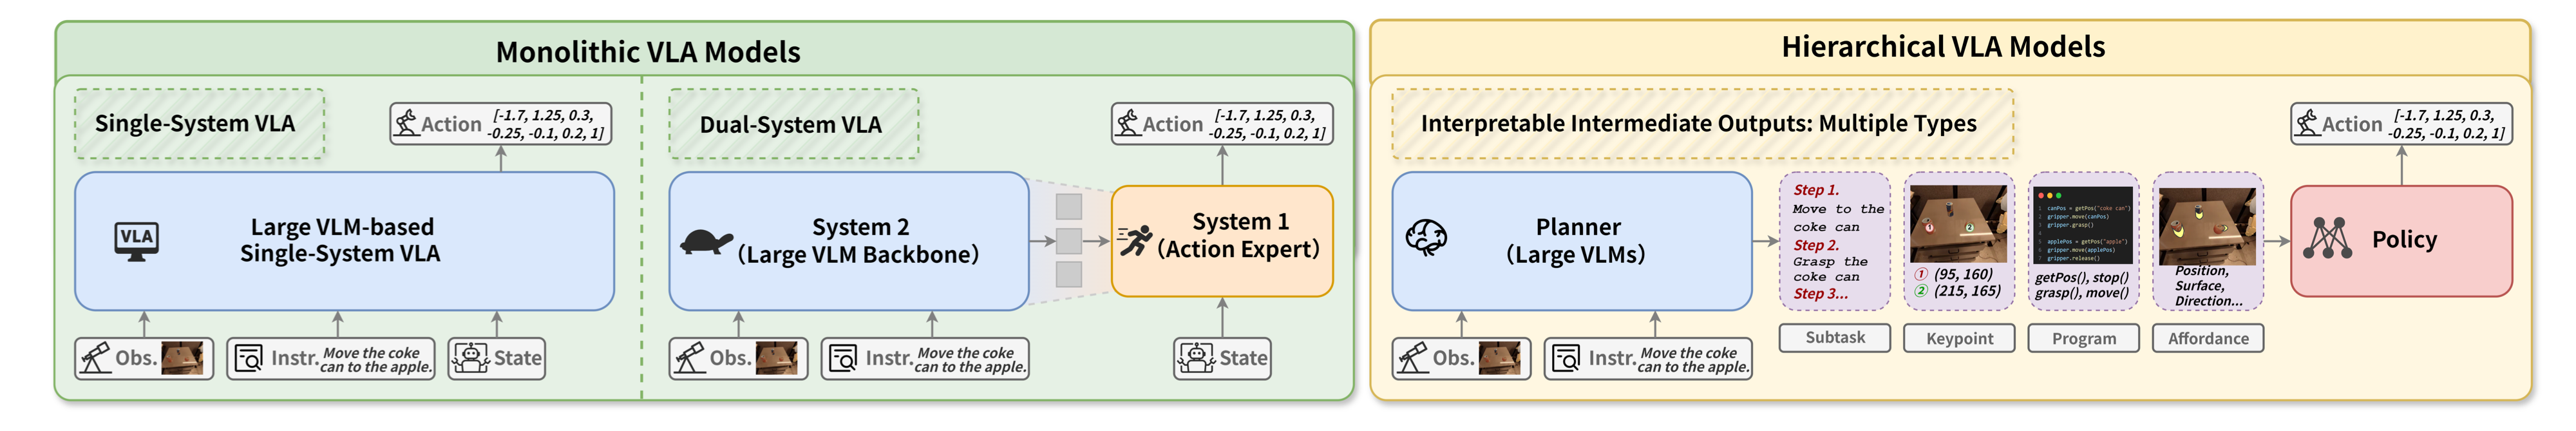
\includegraphics[width=\linewidth]{images/vla-in-robot.png}
    \caption{Comparison between Monolithic and Hierarchical models (from~\cite{vla-in-robot})}
    \label{fig:vla-in-robot}
\end{figure}

Vision-Language-Action (VLA) models are multimodal AI systems that unify visual perception, natural language understanding, and embodied action into a single framework. Originally developed to overcome the fragmentation of traditional robotic pipelines, VLAs integrate pretrained Vision-Language Model (VLM) backbones with action policies, enabling robots to interpret high-level human instructions, reason about spatial relationships, and execute manipulation tasks in dynamic, real-world environments~\cite{vla}. For example, a VLA can follow commands such as “place the red mug next to the laptop onto the top shelf” by grounding visual perception, spatial reasoning, and motor control in a shared computational space. Architecturally, VLAs often rely on transformer-based models that fuse visual, linguistic, and state inputs into a common embedding~\cite{vla},\cite{vla-in-robot}.

A core innovation of VLAs lies in treating robot control as a sequence generation problem. Continuous actions, such as joint angles or end-effector poses, are discretized into tokens, allowing the model to autoregressively predict action tokens in the same way language models generate text. Alongside these, prefix tokens encode context from images and text, while state tokens represent the robot’s internal configuration, as shown in Figure~\ref{fig:vla}. This unified tokenization framework enables reasoning and execution to occur in the same latent space, with a de-tokenizer translating action tokens back into executable motor commands~\cite{vla},\cite{vla-in-robot}.

Two main architectural paradigms have emerged in robotic manipulation, as show in Figure~\ref{fig:vla-in-robot}. Monolithic models directly map multimodal inputs to low-level actions, sometimes combining a “slower” VLM for reasoning with a “faster” policy module for reactive control. In contrast, hierarchical models decouple high-level planning from low-level execution, with a planner producing intermediate representations (e.g., subtasks or keypoints) for downstream policies~\cite{vla-in-robot}. These designs balance efficiency, interpretability, and modularity, depending on task complexity.

VLAs represent a shift from handcrafted pipelines toward end-to-end, language-driven policy generation. They leverage the semantic grounding of VLM pretraining while extending it to action, offering broad potential in robotics, embodied assistants, and human-robot interaction. However, they face limitations such as high computational requirements, difficulty in precisely grounding abstract instructions, and restricted generalization beyond training distributions~\cite{vla},\cite{vla-in-robot}.

\subsection{Planning Domain Definition Language (PDDL)}
\label{sec: pddl}
Planning Domain Definition Language (PDDL) is a standardized language for modeling automated planning problems in artificial intelligence. It separates a domain (the rules of the world: types, predicates, and actions) from a problem (a specific initial state and goal). PDDL allows users to specify objects, predicates, actions, and goals in a structured way, enabling automated planners to generate sequences of actions that achieve desired outcomes. However, PDDL is deliberately neutral: it encodes the physics of a domain without embedding heuristics or solving strategies, meaning many planners only support subsets of the language~\cite{pddl-1.2}.

A classic illustration is the Briefcase World. Here, moving the briefcase also moves everything inside it, while objects can be put in or taken out. Below, the domain defines actions and the problem specifies the goal of moving a dictionary and briefcase to the office while leaving a paycheck at home:

\begin{lstlisting}[language=PDDL]
(define (domain briefcase-world)
  (:requirements :strips :typing :conditional-effects)
  (:types location physob)
  (:constants B - physob)
  (:predicates (at ?x - physob ?l - location) (in ?x ?y - physob))
  (:action mov-b
    :parameters (?m ?l - location)
    :precondition (and (at B ?m) (not (= ?m ?l)))
    :effect (and (at B ?l) (not (at B ?m))
                 (forall (?z)
                   (when (and (in ?z) (not (= ?z B)))
                     (and (at ?z ?l) (not (at ?z ?m)))))))))
  (:action put-in
    :parameters (?x - physob ?l - location)
    :precondition (not (= ?x B))
    :effect (when (and (at ?x ?l) (at B ?l))
                  (in ?x)))
  (:action take-out
    :parameters (?x - physob)
    :precondition (not (= ?x B))
    :effect (not (in ?x)))
                     
(define (problem get-paid)
  (:domain briefcase-world)
  (:init (place home) (place office)
         (object p) (object d) (object b)
         (at B home) (at P home) (at D home) (in P))
  (:goal (and (at B office) (at D office) (at P home))))

\end{lstlisting}

PDDL has evolved from its early versions, like PDDL 1.2, which used predicate logic with true/false properties and actions, to more expressive forms. PDDL 2.1 introduced durative actions and numeric fluents for modeling time and resources, while PDDL 2.2 added derived predicates and timed literals. PDDL 3.0 incorporated soft constraints and preferences with costs, and PDDL+ enabled modeling of processes and uncontrollable events. Specialized variants such as PPDDL, NDDL, and MADDL were later developed for domain-specific planning needs~\cite{pddl}.

\subsection{ROS2}

\begin{figure}[htbp]
    \centering
    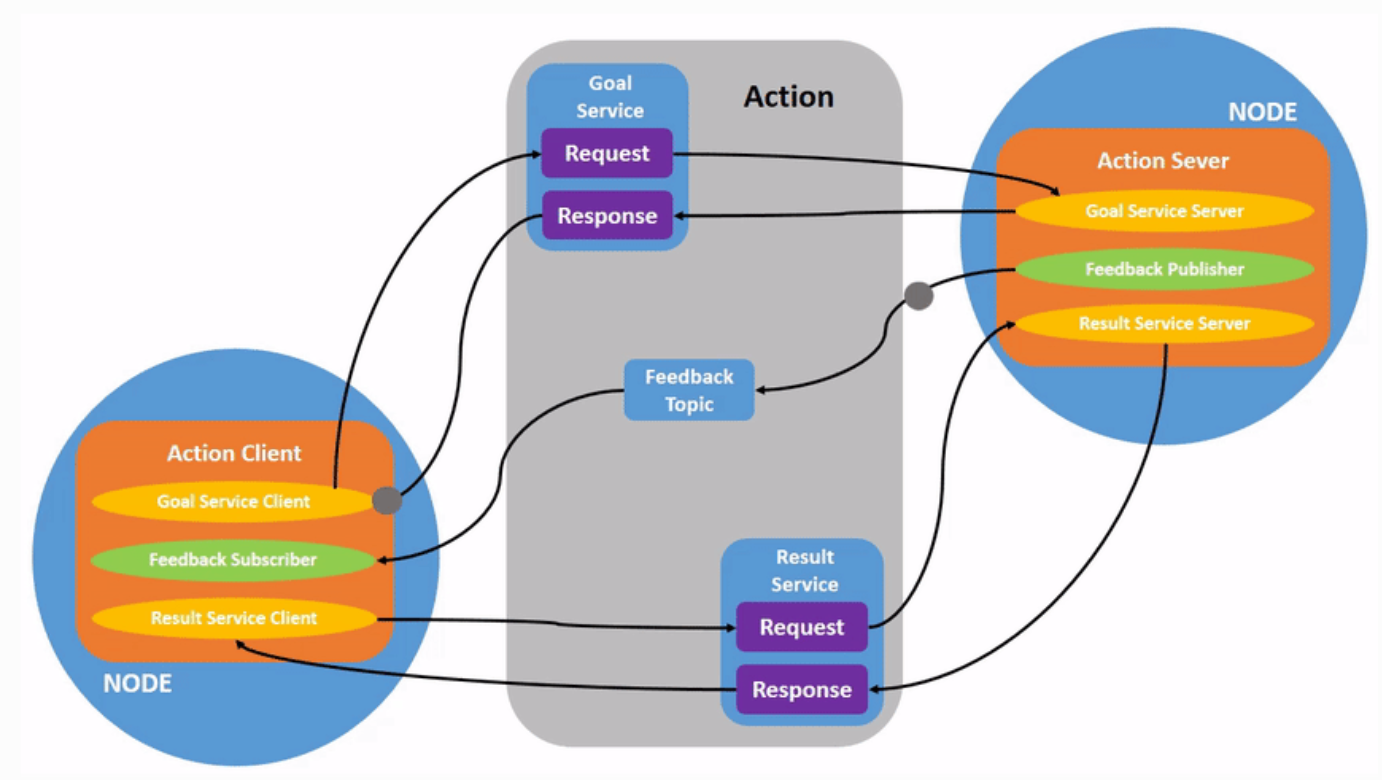
\includegraphics[width=\linewidth]{images/ros2_architecture.png}
    \caption{ROS2 conceptual architecture, illustrating nodes, topics, services, and actions.}
    \label{fig:ros2_architecture}
\end{figure}


ROS2 (Robot Operating System 2) is an open-source middleware framework designed to support the development of distributed, real-time robotic applications. Building upon the foundation of ROS1, ROS2 introduces improved communication paradigms, enhanced reliability, real-time capability, and cross-platform support, making it more suitable for both research and industrial deployment.

At its core, ROS2 is structured around nodes, which are independent processes that communicate through a decentralized publish/subscribe architecture. Nodes exchange messages over topics, invoke synchronous operations through services, and trigger asynchronous long-running tasks via actions. This modular design ensures scalability and flexibility for complex robotic systems. The underlying communication is handled through the Data Distribution Service (DDS), providing discovery, quality-of-service (QoS) policies, and secure data exchange between distributed components.

The ROS2 execution model is further supported by concepts such as parameters for runtime configuration, launch files for orchestrating multiple nodes, and lifecycle management for robust system control. Additionally, the framework introduces tools such as \texttt{ros2cli} for command-line interaction, \texttt{rclcpp}/\texttt{rclpy} for C++ and Python client libraries, and \texttt{rviz2} for visualization. Together, these components form an ecosystem that simplifies robotic software integration while maintaining performance and portability across platforms.

ROS2 represents a shift from experimental middleware to a production-ready robotics framework. Its modularity, DDS-based communication, and lifecycle-aware design provide strong technical backing for robotics research and application development, though challenges such as system complexity and tuning persist~\cite{ros2-doc}.

\subsection{MoveIt2}

MoveIt2 is a motion planning framework for ROS2 that integrates kinematics, collision checking, planning, and execution into a unified pipeline. It enables robots to interpret high-level goals, such as "pick the object and place it in the bin", and compute collision-free, dynamically feasible trajectories to accomplish them.

At its core, MoveIt2 is structured around modular components, as shown in Figure~\ref{fig:moveit_pipeline}. The Kinematics module translates between joint states and end-effector poses, while the Planning Scene Monitor maintains an up-to-date model of the environment. The Motion Planning system leverages planners such as OMPL or TrajOpt to generate valid paths, which are refined in the Trajectory Processing stage into smooth, executable trajectories.

The central move\_group node provides a user-facing API for motion planning and execution, while advanced features like Hybrid Planning combine long-horizon strategies with local reactive control. The MoveIt Task Constructor further extends this capability by composing multi-step task sequences, making it suitable for applications such as bin picking and assembly.

MoveIt2 shifts motion planning from isolated libraries toward a flexible, extensible middleware. Its modular design promotes reusability and adaptability across robotic domains, though challenges remain in accurate modeling, computational cost, and system tuning~\cite{moveit-doc},\cite{moveit2}.

\begin{figure}[htbp]
    \centering
    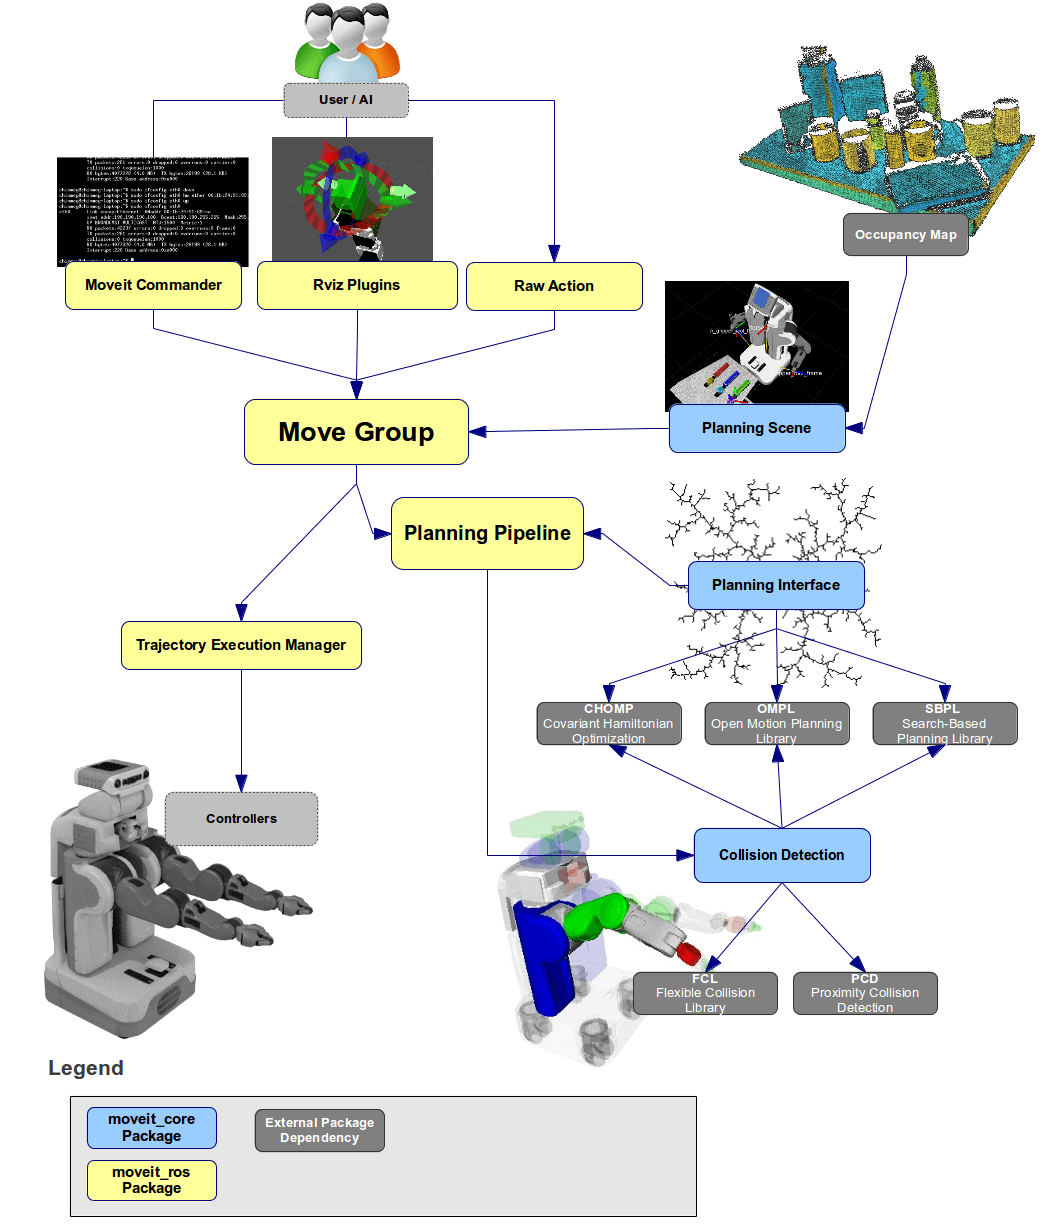
\includegraphics[width=\linewidth]{images/moveit_pipeline.png}
    \caption{MoveIt2 motion planning pipeline.}
    \label{fig:moveit_pipeline}
\end{figure}

\subsection{Gazebo}

Gazebo is an open-source robotics simulation platform that enables realistic, high-fidelity simulation of robots, sensors, and environments. It allows developers to test algorithms, design robots, and train AI models in a virtual setting before deploying on hardware.

Gazebo uses a modular architecture, separating physics, rendering, sensor simulation, and communication. The server handles physics and sensor updates, while the client provides visualization and user interaction. Robots and environments are described using the Simulation Description Format (SDF), and plugins extend functionality for custom behaviors and controllers.

Integrated with ROS, Gazebo allows seamless simulation-to-hardware transitions. Its strengths include realistic physics, sensor modeling, and extensibility through plugins, making it suitable for research, education, and development of both single and multi-robot systems~\cite{gazebo}


\subsection{Artificial Intelligence in Image Processing}

\begin{figure}[htbp]
    \centering
    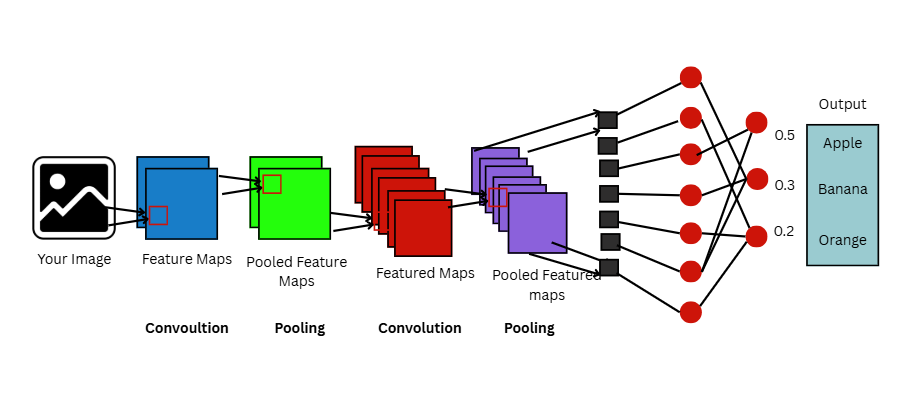
\includegraphics[width=0.8\linewidth]{images/CNN.png}
    \caption{Convolutional Neural Network (CNN) Architecture for Image Classification}
    \label{fig:cnn}
\end{figure}

Artificial Intelligence (AI) has significantly transformed image processing, introducing cutting-edge methods and applications that streamline processes for enhanced speed and accuracy. Image processing itself involves understanding digital images as pixel-based visual information, along with various formats (e.g., JPEG, PNG), enhancement techniques (such as adjusting brightness or reducing noise), and filtering/restoration procedures. Within this framework, AI, especially through deep learning architectures like Convolutional Neural Networks (CNNs) and Generative Adversarial Networks (GANs), enables systems to extract crucial features, recognize objects, segment images, and even generate realistic visual content. This capability allows robots to interpret visual information similarly to humans, finding practical uses in areas like autonomous vehicles for navigation and surveillance systems for security~\cite{ai-in-image-processing}.

The capabilities of AI image processing are broad and impactful, including accuracy enhancements, efficiency improvements, and the capacity to manage large datasets. AI has demonstrated significant success in improving diagnostic accuracy and early disease detection in healthcare, optimizing industrial packing strategies for greater efficiency and reduced waste, and enabling real-time applications and deployment on devices with limited resources through crucial optimization techniques like model compression. Advanced functions such as object detection, image segmentation, and content-based image retrieval are also facilitated by these methods. Despite these advantages, the application of AI in image processing faces notable limitations and ethical challenges. These include critical concerns regarding data privacy, interpretability of AI decisions, and the potential for biases embedded in training data to produce prejudiced results. Therefore, ensuring responsible, transparent AI systems that respect cultural diversity and address potential impacts on employment are vital for the technology's continued development~\cite{ai-in-image-processing}.

\subsection{Universal Robots Arm (UR ARM)}

\begin{figure}[htbp]
    \centering
    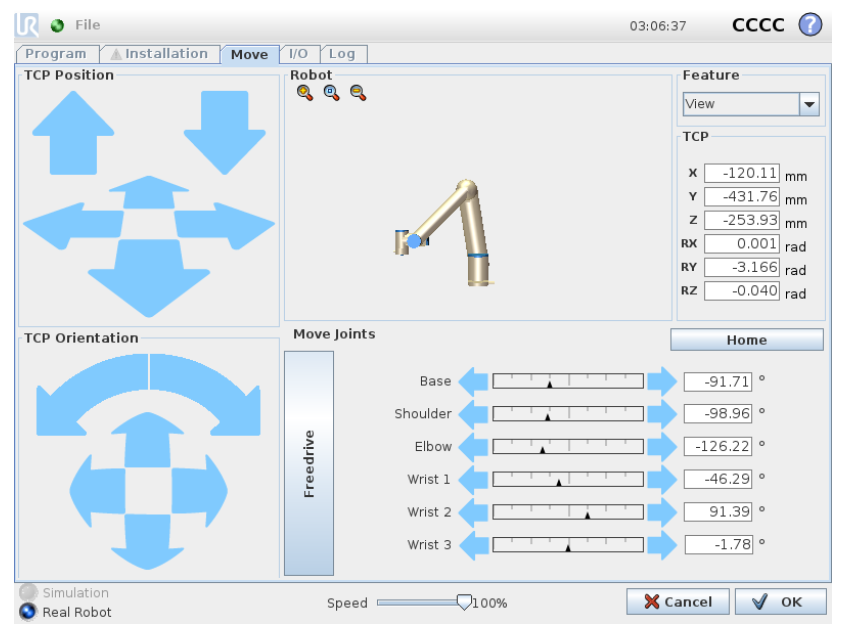
\includegraphics[width=0.8\linewidth]{images/UR_Arm_pic.png}
    \caption{the Move Screen interface of a Universal Robots (UR) robotic arm's ~\cite{urarm}}
    \label{fig:urarm}
\end{figure}

The Universal Robots (UR) robotic arm is a widely adopted collaborative robotic manipulator (cobot) designed for flexible deployment in industrial, engineering, and research settings. Unlike traditional industrial robots, UR arms are specifically engineered to operate safely alongside humans without requiring extensive physical barriers, thanks to their integrated safety features, lightweight design, and force-limiting mechanisms. These properties make UR arms particularly suitable for human-robot collaboration in dynamic environments such as manufacturing, assembly, and tool-handling applications.
From a technical perspective, UR arms employ high-precision servo motors and torque sensors at each joint, enabling six degrees of freedom for dexterous manipulation tasks. Their kinematic flexibility allows execution of both structured and unstructured manipulation tasks, such as grasping, tool usage, and assembly operations. Additionally, UR arms are equipped with programmable interfaces, including graphical user interfaces (GUI), teach pendants, and increasingly, APIs compatible with external AI systems~\cite{urarm}. This enables integration with higher-level control architectures, such as neuro-symbolic AI (NSAI) or large language models (LLMs), for advanced planning, reasoning, and adaptive execution.


\newpage
\section{Project Outcome}

By the deadline of this project , there will be a detailed report documenting how the proposed AI robot arm planning approach performs on the TASK and Motion Planning (TAMP) benchmarks, compared to other baseline solutions. This report will highlight the assistant's strength in combining voice-command understanding, image-processing, and robotic manipulation for engineering tool-handling task.

Accompanying the project is a robotic prototype built on a UR5e robotic arm equipped with a parallel gripper. The robot is connected to a workstation running for UR Arm Library, which serves as the central processing unit, integrating both perception and planning modules. Through this workstation, the robot interfaces with:

\begin{itemize}
    \item \textbf{Camera}:A depth camera for real-time object recognition and workspace mapping.
    \item \textbf{Microphone}: A input with ASR(Automatic Speech Recognition) pipeline for natural voice-command input.
    \item \textbf{Robotics}: Motion controllers for safe execution of grasping and tool-passing tasks. 
\end{itemize}

With these specifications, the prototype is expected to demonstrate the following core capabilities:

\subsection{Autonomous Planning:}

The robot should be able to decompose natural voice instructions (e.g., “pass me the wrench, then place the screwdriver on the table”) into a symbolic task plan and execute it.

\subsubsection{Path and Motion Safety}
The robot should plan trajectories that are collision-free, navigating cluttered tool-workspaces without endangering users or damaging objects.

\subsubsection{Generalization:} The assistant should adapt to unseen scenarios, such as handling tools of unfamiliar shapes or working in rearranged environments, while maintaining performance targets of more than 70 \% sequence correctness and 85 \% collision-free trajectories in simulation when executing TAMP tasks~\cite{tamp}

\subsubsection{Human Collaboration:} The robot must safely pass tools to human collaborators by respecting dynamic human safety zones, pausing or re-planning if a human unexpectedly enters its workspace.

Overall, at the surface level, the outcome of this project will be a robot arm assistant capable of autonomously planning and executing tool-handling tasks in engineering workshop scenarios. On a deeper level, this project demonstrates how combining neural and symbolic AI can produce robots that reason about complex tasks, adapt to novel environments, and safely interact with humans. In the long run, this prototype serves as a foundation for intelligent robotic assistants in manufacturing, laboratories, and educational workshops, showing how autonomous planning can be extended from research into real-world engineering applications.

\newpage
\section{Summary and Benefit to Real Industry}

This project aims to build a prototype of a robotic planning assistant that integrates Large Language Models (LLMs) with symbolic reasoning for tool-handling in engineering environments. The LLM is responsible for translating natural language instructions into multi-step task plans, while Symbolic AI serves as a verification layer, checking for correctness and preventing unsafe or hallucinated actions. The prototype will serve as a proof of concept for how hybrid planning architectures can enable safe, interpretable, and adaptable robotic assistants in industrial settings.

As noted in recent studies~\cite{enhancing-interpret},\cite{learning-neuro-symbolic},\cite{code-as-symbolic-planner},\cite{code-as-policies}, LLMs have demonstrated strong capabilities in task decomposition, code generation, and multimodal integration, while symbolic systems contribute precision, interpretability, and logical consistency ~\cite{code-as-symbolic-planner}. Combining these approaches enhances reliability and operator trust, allowing robots to adapt to unseen scenarios while remaining verifiable.

The expected outcome is a system that reduces downtime, improves safety, and supports human-robot collaboration by enabling robots to be re-tasked directly from natural language instructions without extensive retraining. If successful, this approach can extend beyond tool-handling to applications in \textbf{manufacturing, construction, healthcare, and hazardous environments}, offering a scalable framework for safe and efficient robotic deployment across industries.

\newpage
\section{Roles and Responsibilities}

{
\renewcommand{\arraystretch}{1.3} % 1.3x default row height
\begin{table}[h!]
    \centering
    \begin{tabular}{|l|p{6cm}|l|}
        \hline
        \textbf{Project Task} & \textbf{Task Description} & \textbf{Assigned to} \\
        \hline
        Planning Algorithm & Research architectures, select method, implement, and integrate neuro-symbolic planning algorithm & Kanisorn Sangchai \\
        \hline
        Image Processing & Research techniques, select best method, implement, and integrate image processing for robot system & Methasit Boonpun \\
        \hline
        Speech Processing & Research methods, choose best approach, implement, and integrate speech-to-command module & Withawin Kraipetchara \\
        \hline
        Interface with Robot Arm & Develop UR Arm library, integrate hardware, run simulation, and perform real implementation & Krittin Kitjaruwannakul \\
        \hline
        Project Paperwork & Prepare proposal, progress reports, draft final report, and final presentation & All Members \\
        \hline
    \end{tabular}
    \caption{An outline of major responsibilities assigned to each member within the project}
    \label{tab:roles_responsibilities}
\end{table}
}

The roles and duties of this project revolve around the four main features. Each feature is allocated to a team member as outlined in Table~\ref{tab:roles_responsibilities}


\newpage
\bibliographystyle{IEEEtran}
\bibliography{ref}

\end{document}
